% Options for packages loaded elsewhere
\PassOptionsToPackage{unicode}{hyperref}
\PassOptionsToPackage{hyphens}{url}
%
\documentclass[
  12pt,a4paper,lualatex,ja=standard]{bxjsarticle}
\usepackage{lmodern}
\usepackage{amsmath}
\usepackage{ifxetex,ifluatex}
\ifnum 0\ifxetex 1\fi\ifluatex 1\fi=0 % if pdftex
  \usepackage[T1]{fontenc}
  \usepackage[utf8]{inputenc}
  \usepackage{textcomp} % provide euro and other symbols
  \usepackage{amssymb}
\else % if luatex or xetex
  \usepackage{unicode-math}
  \defaultfontfeatures{Scale=MatchLowercase}
  \defaultfontfeatures[\rmfamily]{Ligatures=TeX,Scale=1}
\fi
% Use upquote if available, for straight quotes in verbatim environments
\IfFileExists{upquote.sty}{\usepackage{upquote}}{}
\IfFileExists{microtype.sty}{% use microtype if available
  \usepackage[]{microtype}
  \UseMicrotypeSet[protrusion]{basicmath} % disable protrusion for tt fonts
}{}
\makeatletter
\@ifundefined{KOMAClassName}{% if non-KOMA class
  \IfFileExists{parskip.sty}{%
    \usepackage{parskip}
  }{% else
    \setlength{\parindent}{0pt}
    \setlength{\parskip}{6pt plus 2pt minus 1pt}}
}{% if KOMA class
  \KOMAoptions{parskip=half}}
\makeatother
\usepackage{xcolor}
\IfFileExists{xurl.sty}{\usepackage{xurl}}{} % add URL line breaks if available
\IfFileExists{bookmark.sty}{\usepackage{bookmark}}{\usepackage{hyperref}}
\hypersetup{
  hidelinks,
  pdfcreator={LaTeX via pandoc}}
\urlstyle{same} % disable monospaced font for URLs
\usepackage{graphicx}
\makeatletter
\def\maxwidth{\ifdim\Gin@nat@width>\linewidth\linewidth\else\Gin@nat@width\fi}
\def\maxheight{\ifdim\Gin@nat@height>\textheight\textheight\else\Gin@nat@height\fi}
\makeatother
% Scale images if necessary, so that they will not overflow the page
% margins by default, and it is still possible to overwrite the defaults
% using explicit options in \includegraphics[width, height, ...]{}
\setkeys{Gin}{width=\maxwidth,height=\maxheight,keepaspectratio}
% Set default figure placement to htbp
\makeatletter
\def\fps@figure{htbp}
\makeatother
\setlength{\emergencystretch}{3em} % prevent overfull lines
\providecommand{\tightlist}{%
  \setlength{\itemsep}{0pt}\setlength{\parskip}{0pt}}
\setcounter{secnumdepth}{5}
\usepackage{indentfirst}
\parindent = 1em
\usepackage{dcolumn}
\newcolumntype{.}{D{.}{.}{-1}}
\usepackage{caption}
\captionsetup[table]{name=表}
\captionsetup[figure]{name=図}
\usepackage{hyperref}
\pagestyle{empty}
\usepackage{multicol}
\usepackage{ascmac}
\setpagelayout*{top=10truemm,bottom=30truemm,left=10truemm,right=10truemm}
\usepackage{tikz}
\usetikzlibrary{arrows.meta,decorations,decorations.pathreplacing,arrows,calc}
\usepackage{tabstackengine}
\usepackage{xcolor}
\usepackage{rotating}
\usepackage{txfonts}
\usepackage{fancybox}
\usepackage{dashbox}
\usepackage{tcolorbox}
\tcbuselibrary{theorems,skins}
\usepackage{siunitx}
\usepackage{framed}
\usepackage{enumerate}
\usepackage{lastpage}
\usepackage{pgfplots}
\pgfplotsset{compat=1.15}
\usepackage{mathrsfs}
\usepackage{pxrubrica}
\ifluatex
  \usepackage{selnolig}  % disable illegal ligatures
\fi

\author{}
\date{\vspace{-2.5em}}

\begin{document}

\renewcommand{\thefootnote}{}
\newcounter{kaunta}
\renewcommand{\thekaunta}{\arabic{kaunta}}
\newcommand{\kaunta}{\refstepcounter{kaunta}%
\thekaunta}
\def\question{\noindent\fbox{\large\makebox[1em]{\text{\kaunta}}} \hspace{1pt}}
\newcounter{skaunta}
\renewcommand{\theskaunta}{\arabic{skaunta}}
\newcommand{\skaunta}{\refstepcounter{skaunta}%
\theskaunta}
\def\squestion{(\text{\skaunta})\hspace{2.5pt}}
\newcommand{\maru}[1]{\raise0.2ex\hbox{\textcircled{\scriptsize{#1}}}}
\newcommand{\jsim}{\mathrel{\text{∽}}}
\newcommand{\jpara}{/\!/}

\newcounter{kcounter}
\setcounter{kcounter}{0}
\newcommand{\kana}{\refstepcounter{kcounter}\ifthenelse{\value{kcounter}=1}{ア}{\ifthenelse{\value{kcounter}=2}{イ}{\ifthenelse{\value{kcounter}=3}{ウ}{\ifthenelse{\value{kcounter}=4}{エ}{\ifthenelse{\value{kcounter}=5}{オ} {\ifthenelse{\value{kcounter}=6}{カ}{\ifthenelse{\value{kcounter}=7}{キ}{\ifthenelse{\value{kcounter}=8}{ク}{\ifthenelse{\value{kcounter}=9}{ケ}{\ifthenelse{\value{kcounter}=10}{コ}{\ifthenelse{\value{kcounter}=11}{サ}{\ifthenelse{\value{kcounter}=12}{シ}{\ifthenelse{\value{kcounter}=13}{ス}{\ifthenelse{\value{kcounter}=14}{セ}{\ifthenelse{\value{kcounter}=15}{ソ}{\ifthenelse{\value{kcounter}=16}{タ}{\ifthenelse{\value{kcounter}=17}{チ}{\ifthenelse{\value{kcounter}=18}{ツ}{\ifthenelse{\value{kcounter}=19}{テ}{\ifthenelse{\value{kcounter}=20}{ト}{\ifthenelse{\value{kcounter}=21}{ナ}{\ifthenelse{\value{kcounter}=22}{ニ}{\ifthenelse{\value{kcounter}=23}{ヌ}{\ifthenelse{\value{kcounter}=24}{ネ}{\ifthenelse{\value{kcounter}=25}{ノ}{\ifthenelse{\value{kcounter}=26}{ハ}{\ifthenelse{\value{kcounter}=27}{ヒ}{\ifthenelse{\value{kcounter}=28}{フ}{\ifthenelse{\value{kcounter}=29}{ヘ}{\ifthenelse{\value{kcounter}=30}{ホ}{\ifthenelse{\value{kcounter}=31}{マ}{\ifthenelse{\value{kcounter}=32}{ミ}{\ifthenelse{\value{kcounter}=33}{ム}{\ifthenelse{\value{kcounter}=34}{メ}{\ifthenelse{\value{kcounter}=35}{モ}{\ifthenelse{\value{kcounter}=36}{ヤ}{\ifthenelse{\value{kcounter}=37}{ユ}{\ifthenelse{\value{kcounter}=38}{ヨ}{\ifthenelse{\value{kcounter}=39}{ラ}{\ifthenelse{\value{kcounter}=40}{リ}{\ifthenelse{\value{kcounter}=41}{ル}{\ifthenelse{\value{kcounter}=42}{レ}{\ifthenelse{\value{kcounter}=43}{ロ}{\ifthenelse{\value{kcounter}=44}{ワ}{・}}}}}}}}}}}}}}}}}}}}}}}}}}}}}}}}}}}}}}}}}}}}}

\newcommand{\kuran}[1]{\framebox[1.5cm][c]{\maru{\kana}}}

\newcommand{\degre}{\ensuremath{^\circ}}

\newcommand{\myarc}[1]{
   \tikz [baseline = (N.base), every node/.style={}] {
      \node [inner sep = 0pt] (N) {$\mathrm{#1}$};
      \draw [line width = 0.4pt] plot [smooth, tension=1.3] coordinates {
         ($(N.north west) + (0.1ex,0)$)
         ($(N.north)      + (0,0.5ex)$)
         ($(N.north east) + (0,0)$)
      };
   }
}

\makeatletter
\newenvironment{figurehere}{\def\@captype{figure}}{}
\makeatother

\newcommand{\haiten}[1]{%
\begin{flushright}%
\footnotesize{<#1>}%
\end{flushright}%
}
\newgeometry{top=10truemm,bottom=10truemm,left=20truemm,right=20truemm}

\thispagestyle{empty}
\begin{center}
\phantom{empty}

\vspace{60truemm}

\hspace{4em} {\HUGE\gtfamily\bfseries \ruby[g]{数}{すう}\hspace{2em}\ruby[g]{学}{がく}}\hspace{1em}{\large \gtfamily \bfseries ($\mathbf{1}$\ruby[g]{年}{ねん})}\\

\vspace{15truemm}

\hspace{2.5em}{\large \gtfamily \bfseries(この\ruby[g]{問題}{もんだい}は\ruby[g]{定規}{じょうぎ}とコンパスが\ruby[g]{必要}{ひつよう}です。)}

\vspace{64truemm}

{\large\gtfamily\bfseries \ruby[g]{注}{ちゅう}\hspace{5em}\ruby[g]{意}{い}}

\end{center}

\centering
\begin{framed}
\begin{flushleft}
\begin{enumerate}[\Large \gtfamily 1]
  \item {\large 「\ruby[g]{開始}{かいし}」の\ruby[g]{合図}{あいず}があるまでは,\ruby[g]{開}{ひら}いてはいけません。}

  \item {\large \ruby[g]{問題}{もんだい}は\pageref{LastPage}ページまであります。}

  \item {\large 「\ruby[g]{開始}{かいし}」の\ruby[g]{合図}{あいず}があったら,まず,\ruby[g]{問題用紙}{もんだいようし}・\ruby[g]{解答用紙}{かいとうようし}に,\ruby[g]{組}{くみ}・\ruby[g]{番号}{ばんごう}と\ruby[g]{名前}{なまえ}などを\ruby[g]{書}{か}きなさい。}

  \item {\large \ruby[g]{答}{こた}えは,すべて\ruby[g]{解答用紙}{かいとうようし}に\ruby[g]{書}{か}きなさい。また、\ruby[g]{所定}{しょてい}の\ruby[g]{欄}{らん}に\ruby[g]{濃}{こ}くはっきりと\ruby[g]{書}{か}きなさい。}

  \item {\large 「\ruby[g]{終了}{しゅうりょう}」の\ruby[g]{合図}{あいず}で,すぐ\ruby[g]{鉛筆}{えんぴつ}をおき,\ruby[g]{解答用紙}{かいとうようし}を\ruby[g]{裏返}{うらがえ}しにしなさい。}
\end{enumerate}
\end{flushleft}
\end{framed}

\vspace{14mm}

\begin{center}
{\large \underline{\hspace{30mm}\ruby[g]{組}{くみ} \hspace{30mm}\ruby[g]{番}{ばん} \hspace{15mm} \ruby[g]{名前}{なまえ} \hspace{60mm}}}
\end{center}

\pagestyle{plain}
\pagenumbering{arabic}

\begin{flushleft}

\noindent\fbox{\large\makebox[1em]{\text{\refstepcounter{kaunta}%
\arabic{kaunta}}}} \hspace{1pt}\ruby[g]{次}{つぎ}の\ruby[g]{空欄}{くうらん}に\ruby[g]{当}{あ}てはまる\ruby[g]{言葉}{ことば}や\ruby[g]{記号}{きごう}を\ruby[g]{書}{か}きなさい。

%
\begin{flushright}%
\footnotesize{<知・技$1 \times 31$点>}%
\end{flushright}%


2\ruby[g]{点}{てん}A, Bを\ruby[g]{通}{とお}り、\ruby[g]{両方}{りょうほう}にかぎりなくのびているものを\framebox[1.5cm][c]{\raise 0.2ex\hbox{\textcircled{\scriptsize{\refstepcounter{kcounter}\ifthenelse{\value{kcounter}=1}{ア}{\ifthenelse{\value{kcounter}=2}{イ}{\ifthenelse{\value{kcounter}=3}{ウ}{\ifthenelse{\value{kcounter}=4}{エ}{\ifthenelse{\value{kcounter}=5}{オ} {\ifthenelse{\value{kcounter}=6}{カ}{\ifthenelse{\value{kcounter}=7}{キ}{\ifthenelse{\value{kcounter}=8}{ク}{\ifthenelse{\value{kcounter}=9}{ケ}{\ifthenelse{\value{kcounter}=10}{コ}{\ifthenelse{\value{kcounter}=11}{サ}{\ifthenelse{\value{kcounter}=12}{シ}{\ifthenelse{\value{kcounter}=13}{ス}{\ifthenelse{\value{kcounter}=14}{セ}{\ifthenelse{\value{kcounter}=15}{ソ}{\ifthenelse{\value{kcounter}=16}{タ}{\ifthenelse{\value{kcounter}=17}{チ}{\ifthenelse{\value{kcounter}=18}{ツ}{\ifthenelse{\value{kcounter}=19}{テ}{\ifthenelse{\value{kcounter}=20}{ト}{\ifthenelse{\value{kcounter}=21}{ナ}{\ifthenelse{\value{kcounter}=22}{ニ}{\ifthenelse{\value{kcounter}=23}{ヌ}{\ifthenelse{\value{kcounter}=24}{ネ}{\ifthenelse{\value{kcounter}=25}{ノ}{\ifthenelse{\value{kcounter}=26}{ハ}{\ifthenelse{\value{kcounter}=27}{ヒ}{\ifthenelse{\value{kcounter}=28}{フ}{\ifthenelse{\value{kcounter}=29}{ヘ}{\ifthenelse{\value{kcounter}=30}{ホ}{\ifthenelse{\value{kcounter}=31}{マ}{\ifthenelse{\value{kcounter}=32}{ミ}{\ifthenelse{\value{kcounter}=33}{ム}{\ifthenelse{\value{kcounter}=34}{メ}{\ifthenelse{\value{kcounter}=35}{モ}{\ifthenelse{\value{kcounter}=36}{ヤ}{\ifthenelse{\value{kcounter}=37}{ユ}{\ifthenelse{\value{kcounter}=38}{ヨ}{\ifthenelse{\value{kcounter}=39}{ラ}{\ifthenelse{\value{kcounter}=40}{リ}{\ifthenelse{\value{kcounter}=41}{ル}{\ifthenelse{\value{kcounter}=42}{レ}{\ifthenelse{\value{kcounter}=43}{ロ}{\ifthenelse{\value{kcounter}=44}{ワ}{・}}}}}}}}}}}}}}}}}}}}}}}}}}}}}}}}}}}}}}}}}}}}}}}}という。\ruby[g]{直線}{ちょくせん}ABのうち、AからBまでの\ruby[g]{部分}{ぶぶん}を\framebox[1.5cm][c]{\raise 0.2ex\hbox{\textcircled{\scriptsize{\refstepcounter{kcounter}\ifthenelse{\value{kcounter}=1}{ア}{\ifthenelse{\value{kcounter}=2}{イ}{\ifthenelse{\value{kcounter}=3}{ウ}{\ifthenelse{\value{kcounter}=4}{エ}{\ifthenelse{\value{kcounter}=5}{オ} {\ifthenelse{\value{kcounter}=6}{カ}{\ifthenelse{\value{kcounter}=7}{キ}{\ifthenelse{\value{kcounter}=8}{ク}{\ifthenelse{\value{kcounter}=9}{ケ}{\ifthenelse{\value{kcounter}=10}{コ}{\ifthenelse{\value{kcounter}=11}{サ}{\ifthenelse{\value{kcounter}=12}{シ}{\ifthenelse{\value{kcounter}=13}{ス}{\ifthenelse{\value{kcounter}=14}{セ}{\ifthenelse{\value{kcounter}=15}{ソ}{\ifthenelse{\value{kcounter}=16}{タ}{\ifthenelse{\value{kcounter}=17}{チ}{\ifthenelse{\value{kcounter}=18}{ツ}{\ifthenelse{\value{kcounter}=19}{テ}{\ifthenelse{\value{kcounter}=20}{ト}{\ifthenelse{\value{kcounter}=21}{ナ}{\ifthenelse{\value{kcounter}=22}{ニ}{\ifthenelse{\value{kcounter}=23}{ヌ}{\ifthenelse{\value{kcounter}=24}{ネ}{\ifthenelse{\value{kcounter}=25}{ノ}{\ifthenelse{\value{kcounter}=26}{ハ}{\ifthenelse{\value{kcounter}=27}{ヒ}{\ifthenelse{\value{kcounter}=28}{フ}{\ifthenelse{\value{kcounter}=29}{ヘ}{\ifthenelse{\value{kcounter}=30}{ホ}{\ifthenelse{\value{kcounter}=31}{マ}{\ifthenelse{\value{kcounter}=32}{ミ}{\ifthenelse{\value{kcounter}=33}{ム}{\ifthenelse{\value{kcounter}=34}{メ}{\ifthenelse{\value{kcounter}=35}{モ}{\ifthenelse{\value{kcounter}=36}{ヤ}{\ifthenelse{\value{kcounter}=37}{ユ}{\ifthenelse{\value{kcounter}=38}{ヨ}{\ifthenelse{\value{kcounter}=39}{ラ}{\ifthenelse{\value{kcounter}=40}{リ}{\ifthenelse{\value{kcounter}=41}{ル}{\ifthenelse{\value{kcounter}=42}{レ}{\ifthenelse{\value{kcounter}=43}{ロ}{\ifthenelse{\value{kcounter}=44}{ワ}{・}}}}}}}}}}}}}}}}}}}}}}}}}}}}}}}}}}}}}}}}}}}}}}}}という。また、\ruby[g]{線分}{せんぶん}ABをBのほうへまっすぐにかぎりなくのばしたものを\framebox[1.5cm][c]{\raise 0.2ex\hbox{\textcircled{\scriptsize{\refstepcounter{kcounter}\ifthenelse{\value{kcounter}=1}{ア}{\ifthenelse{\value{kcounter}=2}{イ}{\ifthenelse{\value{kcounter}=3}{ウ}{\ifthenelse{\value{kcounter}=4}{エ}{\ifthenelse{\value{kcounter}=5}{オ} {\ifthenelse{\value{kcounter}=6}{カ}{\ifthenelse{\value{kcounter}=7}{キ}{\ifthenelse{\value{kcounter}=8}{ク}{\ifthenelse{\value{kcounter}=9}{ケ}{\ifthenelse{\value{kcounter}=10}{コ}{\ifthenelse{\value{kcounter}=11}{サ}{\ifthenelse{\value{kcounter}=12}{シ}{\ifthenelse{\value{kcounter}=13}{ス}{\ifthenelse{\value{kcounter}=14}{セ}{\ifthenelse{\value{kcounter}=15}{ソ}{\ifthenelse{\value{kcounter}=16}{タ}{\ifthenelse{\value{kcounter}=17}{チ}{\ifthenelse{\value{kcounter}=18}{ツ}{\ifthenelse{\value{kcounter}=19}{テ}{\ifthenelse{\value{kcounter}=20}{ト}{\ifthenelse{\value{kcounter}=21}{ナ}{\ifthenelse{\value{kcounter}=22}{ニ}{\ifthenelse{\value{kcounter}=23}{ヌ}{\ifthenelse{\value{kcounter}=24}{ネ}{\ifthenelse{\value{kcounter}=25}{ノ}{\ifthenelse{\value{kcounter}=26}{ハ}{\ifthenelse{\value{kcounter}=27}{ヒ}{\ifthenelse{\value{kcounter}=28}{フ}{\ifthenelse{\value{kcounter}=29}{ヘ}{\ifthenelse{\value{kcounter}=30}{ホ}{\ifthenelse{\value{kcounter}=31}{マ}{\ifthenelse{\value{kcounter}=32}{ミ}{\ifthenelse{\value{kcounter}=33}{ム}{\ifthenelse{\value{kcounter}=34}{メ}{\ifthenelse{\value{kcounter}=35}{モ}{\ifthenelse{\value{kcounter}=36}{ヤ}{\ifthenelse{\value{kcounter}=37}{ユ}{\ifthenelse{\value{kcounter}=38}{ヨ}{\ifthenelse{\value{kcounter}=39}{ラ}{\ifthenelse{\value{kcounter}=40}{リ}{\ifthenelse{\value{kcounter}=41}{ル}{\ifthenelse{\value{kcounter}=42}{レ}{\ifthenelse{\value{kcounter}=43}{ロ}{\ifthenelse{\value{kcounter}=44}{ワ}{・}}}}}}}}}}}}}}}}}}}}}}}}}}}}}}}}}}}}}}}}}}}}}}}}という。

\ruby[g]{図形}{ずけい}を、\ruby[g]{一定}{いってい}の\ruby[g]{方向}{ほうこう}に、\ruby[g]{一定}{いってい}の\ruby[g]{距離}{きょり}だけ\ruby[g]{動}{うご}かす\ruby[g]{移動}{いどう}を\framebox[1.5cm][c]{\raise 0.2ex\hbox{\textcircled{\scriptsize{\refstepcounter{kcounter}\ifthenelse{\value{kcounter}=1}{ア}{\ifthenelse{\value{kcounter}=2}{イ}{\ifthenelse{\value{kcounter}=3}{ウ}{\ifthenelse{\value{kcounter}=4}{エ}{\ifthenelse{\value{kcounter}=5}{オ} {\ifthenelse{\value{kcounter}=6}{カ}{\ifthenelse{\value{kcounter}=7}{キ}{\ifthenelse{\value{kcounter}=8}{ク}{\ifthenelse{\value{kcounter}=9}{ケ}{\ifthenelse{\value{kcounter}=10}{コ}{\ifthenelse{\value{kcounter}=11}{サ}{\ifthenelse{\value{kcounter}=12}{シ}{\ifthenelse{\value{kcounter}=13}{ス}{\ifthenelse{\value{kcounter}=14}{セ}{\ifthenelse{\value{kcounter}=15}{ソ}{\ifthenelse{\value{kcounter}=16}{タ}{\ifthenelse{\value{kcounter}=17}{チ}{\ifthenelse{\value{kcounter}=18}{ツ}{\ifthenelse{\value{kcounter}=19}{テ}{\ifthenelse{\value{kcounter}=20}{ト}{\ifthenelse{\value{kcounter}=21}{ナ}{\ifthenelse{\value{kcounter}=22}{ニ}{\ifthenelse{\value{kcounter}=23}{ヌ}{\ifthenelse{\value{kcounter}=24}{ネ}{\ifthenelse{\value{kcounter}=25}{ノ}{\ifthenelse{\value{kcounter}=26}{ハ}{\ifthenelse{\value{kcounter}=27}{ヒ}{\ifthenelse{\value{kcounter}=28}{フ}{\ifthenelse{\value{kcounter}=29}{ヘ}{\ifthenelse{\value{kcounter}=30}{ホ}{\ifthenelse{\value{kcounter}=31}{マ}{\ifthenelse{\value{kcounter}=32}{ミ}{\ifthenelse{\value{kcounter}=33}{ム}{\ifthenelse{\value{kcounter}=34}{メ}{\ifthenelse{\value{kcounter}=35}{モ}{\ifthenelse{\value{kcounter}=36}{ヤ}{\ifthenelse{\value{kcounter}=37}{ユ}{\ifthenelse{\value{kcounter}=38}{ヨ}{\ifthenelse{\value{kcounter}=39}{ラ}{\ifthenelse{\value{kcounter}=40}{リ}{\ifthenelse{\value{kcounter}=41}{ル}{\ifthenelse{\value{kcounter}=42}{レ}{\ifthenelse{\value{kcounter}=43}{ロ}{\ifthenelse{\value{kcounter}=44}{ワ}{・}}}}}}}}}}}}}}}}}}}}}}}}}}}}}}}}}}}}}}}}}}}}}}}}という。\ruby[g]{線分}{せんぶん}ABと\ruby[g]{線分}{せんぶん}CDの\ruby[g]{長}{なが}さが\ruby[g]{等}{ひと}しいことをAB \framebox[1.5cm][c]{\raise 0.2ex\hbox{\textcircled{\scriptsize{\refstepcounter{kcounter}\ifthenelse{\value{kcounter}=1}{ア}{\ifthenelse{\value{kcounter}=2}{イ}{\ifthenelse{\value{kcounter}=3}{ウ}{\ifthenelse{\value{kcounter}=4}{エ}{\ifthenelse{\value{kcounter}=5}{オ} {\ifthenelse{\value{kcounter}=6}{カ}{\ifthenelse{\value{kcounter}=7}{キ}{\ifthenelse{\value{kcounter}=8}{ク}{\ifthenelse{\value{kcounter}=9}{ケ}{\ifthenelse{\value{kcounter}=10}{コ}{\ifthenelse{\value{kcounter}=11}{サ}{\ifthenelse{\value{kcounter}=12}{シ}{\ifthenelse{\value{kcounter}=13}{ス}{\ifthenelse{\value{kcounter}=14}{セ}{\ifthenelse{\value{kcounter}=15}{ソ}{\ifthenelse{\value{kcounter}=16}{タ}{\ifthenelse{\value{kcounter}=17}{チ}{\ifthenelse{\value{kcounter}=18}{ツ}{\ifthenelse{\value{kcounter}=19}{テ}{\ifthenelse{\value{kcounter}=20}{ト}{\ifthenelse{\value{kcounter}=21}{ナ}{\ifthenelse{\value{kcounter}=22}{ニ}{\ifthenelse{\value{kcounter}=23}{ヌ}{\ifthenelse{\value{kcounter}=24}{ネ}{\ifthenelse{\value{kcounter}=25}{ノ}{\ifthenelse{\value{kcounter}=26}{ハ}{\ifthenelse{\value{kcounter}=27}{ヒ}{\ifthenelse{\value{kcounter}=28}{フ}{\ifthenelse{\value{kcounter}=29}{ヘ}{\ifthenelse{\value{kcounter}=30}{ホ}{\ifthenelse{\value{kcounter}=31}{マ}{\ifthenelse{\value{kcounter}=32}{ミ}{\ifthenelse{\value{kcounter}=33}{ム}{\ifthenelse{\value{kcounter}=34}{メ}{\ifthenelse{\value{kcounter}=35}{モ}{\ifthenelse{\value{kcounter}=36}{ヤ}{\ifthenelse{\value{kcounter}=37}{ユ}{\ifthenelse{\value{kcounter}=38}{ヨ}{\ifthenelse{\value{kcounter}=39}{ラ}{\ifthenelse{\value{kcounter}=40}{リ}{\ifthenelse{\value{kcounter}=41}{ル}{\ifthenelse{\value{kcounter}=42}{レ}{\ifthenelse{\value{kcounter}=43}{ロ}{\ifthenelse{\value{kcounter}=44}{ワ}{・}}}}}}}}}}}}}}}}}}}}}}}}}}}}}}}}}}}}}}}}}}}}}}}} CDとかく。\ruby[g]{図形}{ずけい}をある\ruby[g]{点}{てん}を\ruby[g]{中心}{ちゅうしん}として、\ruby[g]{一定}{いってい}の\ruby[g]{角度}{かくど}だけ\ruby[g]{回転}{かいてん}させる\ruby[g]{移動}{いどう}を\framebox[1.5cm][c]{\raise 0.2ex\hbox{\textcircled{\scriptsize{\refstepcounter{kcounter}\ifthenelse{\value{kcounter}=1}{ア}{\ifthenelse{\value{kcounter}=2}{イ}{\ifthenelse{\value{kcounter}=3}{ウ}{\ifthenelse{\value{kcounter}=4}{エ}{\ifthenelse{\value{kcounter}=5}{オ} {\ifthenelse{\value{kcounter}=6}{カ}{\ifthenelse{\value{kcounter}=7}{キ}{\ifthenelse{\value{kcounter}=8}{ク}{\ifthenelse{\value{kcounter}=9}{ケ}{\ifthenelse{\value{kcounter}=10}{コ}{\ifthenelse{\value{kcounter}=11}{サ}{\ifthenelse{\value{kcounter}=12}{シ}{\ifthenelse{\value{kcounter}=13}{ス}{\ifthenelse{\value{kcounter}=14}{セ}{\ifthenelse{\value{kcounter}=15}{ソ}{\ifthenelse{\value{kcounter}=16}{タ}{\ifthenelse{\value{kcounter}=17}{チ}{\ifthenelse{\value{kcounter}=18}{ツ}{\ifthenelse{\value{kcounter}=19}{テ}{\ifthenelse{\value{kcounter}=20}{ト}{\ifthenelse{\value{kcounter}=21}{ナ}{\ifthenelse{\value{kcounter}=22}{ニ}{\ifthenelse{\value{kcounter}=23}{ヌ}{\ifthenelse{\value{kcounter}=24}{ネ}{\ifthenelse{\value{kcounter}=25}{ノ}{\ifthenelse{\value{kcounter}=26}{ハ}{\ifthenelse{\value{kcounter}=27}{ヒ}{\ifthenelse{\value{kcounter}=28}{フ}{\ifthenelse{\value{kcounter}=29}{ヘ}{\ifthenelse{\value{kcounter}=30}{ホ}{\ifthenelse{\value{kcounter}=31}{マ}{\ifthenelse{\value{kcounter}=32}{ミ}{\ifthenelse{\value{kcounter}=33}{ム}{\ifthenelse{\value{kcounter}=34}{メ}{\ifthenelse{\value{kcounter}=35}{モ}{\ifthenelse{\value{kcounter}=36}{ヤ}{\ifthenelse{\value{kcounter}=37}{ユ}{\ifthenelse{\value{kcounter}=38}{ヨ}{\ifthenelse{\value{kcounter}=39}{ラ}{\ifthenelse{\value{kcounter}=40}{リ}{\ifthenelse{\value{kcounter}=41}{ル}{\ifthenelse{\value{kcounter}=42}{レ}{\ifthenelse{\value{kcounter}=43}{ロ}{\ifthenelse{\value{kcounter}=44}{ワ}{・}}}}}}}}}}}}}}}}}}}}}}}}}}}}}}}}}}}}}}}}}}}}}}}}といい、\ruby[g]{中心}{ちゅうしん}とする\ruby[g]{点}{てん}を\framebox[1.5cm][c]{\raise 0.2ex\hbox{\textcircled{\scriptsize{\refstepcounter{kcounter}\ifthenelse{\value{kcounter}=1}{ア}{\ifthenelse{\value{kcounter}=2}{イ}{\ifthenelse{\value{kcounter}=3}{ウ}{\ifthenelse{\value{kcounter}=4}{エ}{\ifthenelse{\value{kcounter}=5}{オ} {\ifthenelse{\value{kcounter}=6}{カ}{\ifthenelse{\value{kcounter}=7}{キ}{\ifthenelse{\value{kcounter}=8}{ク}{\ifthenelse{\value{kcounter}=9}{ケ}{\ifthenelse{\value{kcounter}=10}{コ}{\ifthenelse{\value{kcounter}=11}{サ}{\ifthenelse{\value{kcounter}=12}{シ}{\ifthenelse{\value{kcounter}=13}{ス}{\ifthenelse{\value{kcounter}=14}{セ}{\ifthenelse{\value{kcounter}=15}{ソ}{\ifthenelse{\value{kcounter}=16}{タ}{\ifthenelse{\value{kcounter}=17}{チ}{\ifthenelse{\value{kcounter}=18}{ツ}{\ifthenelse{\value{kcounter}=19}{テ}{\ifthenelse{\value{kcounter}=20}{ト}{\ifthenelse{\value{kcounter}=21}{ナ}{\ifthenelse{\value{kcounter}=22}{ニ}{\ifthenelse{\value{kcounter}=23}{ヌ}{\ifthenelse{\value{kcounter}=24}{ネ}{\ifthenelse{\value{kcounter}=25}{ノ}{\ifthenelse{\value{kcounter}=26}{ハ}{\ifthenelse{\value{kcounter}=27}{ヒ}{\ifthenelse{\value{kcounter}=28}{フ}{\ifthenelse{\value{kcounter}=29}{ヘ}{\ifthenelse{\value{kcounter}=30}{ホ}{\ifthenelse{\value{kcounter}=31}{マ}{\ifthenelse{\value{kcounter}=32}{ミ}{\ifthenelse{\value{kcounter}=33}{ム}{\ifthenelse{\value{kcounter}=34}{メ}{\ifthenelse{\value{kcounter}=35}{モ}{\ifthenelse{\value{kcounter}=36}{ヤ}{\ifthenelse{\value{kcounter}=37}{ユ}{\ifthenelse{\value{kcounter}=38}{ヨ}{\ifthenelse{\value{kcounter}=39}{ラ}{\ifthenelse{\value{kcounter}=40}{リ}{\ifthenelse{\value{kcounter}=41}{ル}{\ifthenelse{\value{kcounter}=42}{レ}{\ifthenelse{\value{kcounter}=43}{ロ}{\ifthenelse{\value{kcounter}=44}{ワ}{・}}}}}}}}}}}}}}}}}}}}}}}}}}}}}}}}}}}}}}}}}}}}}}}}という。\ruby[g]{図形}{ずけい}を$\ang{180}$だけ\ruby[g]{回転移動}{かいてんいどう}させることを\framebox[1.5cm][c]{\raise 0.2ex\hbox{\textcircled{\scriptsize{\refstepcounter{kcounter}\ifthenelse{\value{kcounter}=1}{ア}{\ifthenelse{\value{kcounter}=2}{イ}{\ifthenelse{\value{kcounter}=3}{ウ}{\ifthenelse{\value{kcounter}=4}{エ}{\ifthenelse{\value{kcounter}=5}{オ} {\ifthenelse{\value{kcounter}=6}{カ}{\ifthenelse{\value{kcounter}=7}{キ}{\ifthenelse{\value{kcounter}=8}{ク}{\ifthenelse{\value{kcounter}=9}{ケ}{\ifthenelse{\value{kcounter}=10}{コ}{\ifthenelse{\value{kcounter}=11}{サ}{\ifthenelse{\value{kcounter}=12}{シ}{\ifthenelse{\value{kcounter}=13}{ス}{\ifthenelse{\value{kcounter}=14}{セ}{\ifthenelse{\value{kcounter}=15}{ソ}{\ifthenelse{\value{kcounter}=16}{タ}{\ifthenelse{\value{kcounter}=17}{チ}{\ifthenelse{\value{kcounter}=18}{ツ}{\ifthenelse{\value{kcounter}=19}{テ}{\ifthenelse{\value{kcounter}=20}{ト}{\ifthenelse{\value{kcounter}=21}{ナ}{\ifthenelse{\value{kcounter}=22}{ニ}{\ifthenelse{\value{kcounter}=23}{ヌ}{\ifthenelse{\value{kcounter}=24}{ネ}{\ifthenelse{\value{kcounter}=25}{ノ}{\ifthenelse{\value{kcounter}=26}{ハ}{\ifthenelse{\value{kcounter}=27}{ヒ}{\ifthenelse{\value{kcounter}=28}{フ}{\ifthenelse{\value{kcounter}=29}{ヘ}{\ifthenelse{\value{kcounter}=30}{ホ}{\ifthenelse{\value{kcounter}=31}{マ}{\ifthenelse{\value{kcounter}=32}{ミ}{\ifthenelse{\value{kcounter}=33}{ム}{\ifthenelse{\value{kcounter}=34}{メ}{\ifthenelse{\value{kcounter}=35}{モ}{\ifthenelse{\value{kcounter}=36}{ヤ}{\ifthenelse{\value{kcounter}=37}{ユ}{\ifthenelse{\value{kcounter}=38}{ヨ}{\ifthenelse{\value{kcounter}=39}{ラ}{\ifthenelse{\value{kcounter}=40}{リ}{\ifthenelse{\value{kcounter}=41}{ル}{\ifthenelse{\value{kcounter}=42}{レ}{\ifthenelse{\value{kcounter}=43}{ロ}{\ifthenelse{\value{kcounter}=44}{ワ}{・}}}}}}}}}}}}}}}}}}}}}}}}}}}}}}}}}}}}}}}}}}}}}}}}という。また、\ruby[g]{図形}{ずけい}をある\ruby[g]{直線}{ちょくせん}を\ruby[g]{折}{お}り\ruby[g]{目}{め}として\ruby[g]{折}{お}り\ruby[g]{返}{かえ}す\ruby[g]{移動}{いどう}を\framebox[1.5cm][c]{\raise 0.2ex\hbox{\textcircled{\scriptsize{\refstepcounter{kcounter}\ifthenelse{\value{kcounter}=1}{ア}{\ifthenelse{\value{kcounter}=2}{イ}{\ifthenelse{\value{kcounter}=3}{ウ}{\ifthenelse{\value{kcounter}=4}{エ}{\ifthenelse{\value{kcounter}=5}{オ} {\ifthenelse{\value{kcounter}=6}{カ}{\ifthenelse{\value{kcounter}=7}{キ}{\ifthenelse{\value{kcounter}=8}{ク}{\ifthenelse{\value{kcounter}=9}{ケ}{\ifthenelse{\value{kcounter}=10}{コ}{\ifthenelse{\value{kcounter}=11}{サ}{\ifthenelse{\value{kcounter}=12}{シ}{\ifthenelse{\value{kcounter}=13}{ス}{\ifthenelse{\value{kcounter}=14}{セ}{\ifthenelse{\value{kcounter}=15}{ソ}{\ifthenelse{\value{kcounter}=16}{タ}{\ifthenelse{\value{kcounter}=17}{チ}{\ifthenelse{\value{kcounter}=18}{ツ}{\ifthenelse{\value{kcounter}=19}{テ}{\ifthenelse{\value{kcounter}=20}{ト}{\ifthenelse{\value{kcounter}=21}{ナ}{\ifthenelse{\value{kcounter}=22}{ニ}{\ifthenelse{\value{kcounter}=23}{ヌ}{\ifthenelse{\value{kcounter}=24}{ネ}{\ifthenelse{\value{kcounter}=25}{ノ}{\ifthenelse{\value{kcounter}=26}{ハ}{\ifthenelse{\value{kcounter}=27}{ヒ}{\ifthenelse{\value{kcounter}=28}{フ}{\ifthenelse{\value{kcounter}=29}{ヘ}{\ifthenelse{\value{kcounter}=30}{ホ}{\ifthenelse{\value{kcounter}=31}{マ}{\ifthenelse{\value{kcounter}=32}{ミ}{\ifthenelse{\value{kcounter}=33}{ム}{\ifthenelse{\value{kcounter}=34}{メ}{\ifthenelse{\value{kcounter}=35}{モ}{\ifthenelse{\value{kcounter}=36}{ヤ}{\ifthenelse{\value{kcounter}=37}{ユ}{\ifthenelse{\value{kcounter}=38}{ヨ}{\ifthenelse{\value{kcounter}=39}{ラ}{\ifthenelse{\value{kcounter}=40}{リ}{\ifthenelse{\value{kcounter}=41}{ル}{\ifthenelse{\value{kcounter}=42}{レ}{\ifthenelse{\value{kcounter}=43}{ロ}{\ifthenelse{\value{kcounter}=44}{ワ}{・}}}}}}}}}}}}}}}}}}}}}}}}}}}}}}}}}}}}}}}}}}}}}}}}といい、\ruby[g]{折}{お}り\ruby[g]{目}{め}の\ruby[g]{直線}{ちょくせん}を\framebox[1.5cm][c]{\raise 0.2ex\hbox{\textcircled{\scriptsize{\refstepcounter{kcounter}\ifthenelse{\value{kcounter}=1}{ア}{\ifthenelse{\value{kcounter}=2}{イ}{\ifthenelse{\value{kcounter}=3}{ウ}{\ifthenelse{\value{kcounter}=4}{エ}{\ifthenelse{\value{kcounter}=5}{オ} {\ifthenelse{\value{kcounter}=6}{カ}{\ifthenelse{\value{kcounter}=7}{キ}{\ifthenelse{\value{kcounter}=8}{ク}{\ifthenelse{\value{kcounter}=9}{ケ}{\ifthenelse{\value{kcounter}=10}{コ}{\ifthenelse{\value{kcounter}=11}{サ}{\ifthenelse{\value{kcounter}=12}{シ}{\ifthenelse{\value{kcounter}=13}{ス}{\ifthenelse{\value{kcounter}=14}{セ}{\ifthenelse{\value{kcounter}=15}{ソ}{\ifthenelse{\value{kcounter}=16}{タ}{\ifthenelse{\value{kcounter}=17}{チ}{\ifthenelse{\value{kcounter}=18}{ツ}{\ifthenelse{\value{kcounter}=19}{テ}{\ifthenelse{\value{kcounter}=20}{ト}{\ifthenelse{\value{kcounter}=21}{ナ}{\ifthenelse{\value{kcounter}=22}{ニ}{\ifthenelse{\value{kcounter}=23}{ヌ}{\ifthenelse{\value{kcounter}=24}{ネ}{\ifthenelse{\value{kcounter}=25}{ノ}{\ifthenelse{\value{kcounter}=26}{ハ}{\ifthenelse{\value{kcounter}=27}{ヒ}{\ifthenelse{\value{kcounter}=28}{フ}{\ifthenelse{\value{kcounter}=29}{ヘ}{\ifthenelse{\value{kcounter}=30}{ホ}{\ifthenelse{\value{kcounter}=31}{マ}{\ifthenelse{\value{kcounter}=32}{ミ}{\ifthenelse{\value{kcounter}=33}{ム}{\ifthenelse{\value{kcounter}=34}{メ}{\ifthenelse{\value{kcounter}=35}{モ}{\ifthenelse{\value{kcounter}=36}{ヤ}{\ifthenelse{\value{kcounter}=37}{ユ}{\ifthenelse{\value{kcounter}=38}{ヨ}{\ifthenelse{\value{kcounter}=39}{ラ}{\ifthenelse{\value{kcounter}=40}{リ}{\ifthenelse{\value{kcounter}=41}{ル}{\ifthenelse{\value{kcounter}=42}{レ}{\ifthenelse{\value{kcounter}=43}{ロ}{\ifthenelse{\value{kcounter}=44}{ワ}{・}}}}}}}}}}}}}}}}}}}}}}}}}}}}}}}}}}}}}}}}}}}}}}}}という。

\ruby[g]{平行}{へいこう}な2\ruby[g]{直線}{ちょくせん}を\framebox[1.5cm][c]{\raise 0.2ex\hbox{\textcircled{\scriptsize{\refstepcounter{kcounter}\ifthenelse{\value{kcounter}=1}{ア}{\ifthenelse{\value{kcounter}=2}{イ}{\ifthenelse{\value{kcounter}=3}{ウ}{\ifthenelse{\value{kcounter}=4}{エ}{\ifthenelse{\value{kcounter}=5}{オ} {\ifthenelse{\value{kcounter}=6}{カ}{\ifthenelse{\value{kcounter}=7}{キ}{\ifthenelse{\value{kcounter}=8}{ク}{\ifthenelse{\value{kcounter}=9}{ケ}{\ifthenelse{\value{kcounter}=10}{コ}{\ifthenelse{\value{kcounter}=11}{サ}{\ifthenelse{\value{kcounter}=12}{シ}{\ifthenelse{\value{kcounter}=13}{ス}{\ifthenelse{\value{kcounter}=14}{セ}{\ifthenelse{\value{kcounter}=15}{ソ}{\ifthenelse{\value{kcounter}=16}{タ}{\ifthenelse{\value{kcounter}=17}{チ}{\ifthenelse{\value{kcounter}=18}{ツ}{\ifthenelse{\value{kcounter}=19}{テ}{\ifthenelse{\value{kcounter}=20}{ト}{\ifthenelse{\value{kcounter}=21}{ナ}{\ifthenelse{\value{kcounter}=22}{ニ}{\ifthenelse{\value{kcounter}=23}{ヌ}{\ifthenelse{\value{kcounter}=24}{ネ}{\ifthenelse{\value{kcounter}=25}{ノ}{\ifthenelse{\value{kcounter}=26}{ハ}{\ifthenelse{\value{kcounter}=27}{ヒ}{\ifthenelse{\value{kcounter}=28}{フ}{\ifthenelse{\value{kcounter}=29}{ヘ}{\ifthenelse{\value{kcounter}=30}{ホ}{\ifthenelse{\value{kcounter}=31}{マ}{\ifthenelse{\value{kcounter}=32}{ミ}{\ifthenelse{\value{kcounter}=33}{ム}{\ifthenelse{\value{kcounter}=34}{メ}{\ifthenelse{\value{kcounter}=35}{モ}{\ifthenelse{\value{kcounter}=36}{ヤ}{\ifthenelse{\value{kcounter}=37}{ユ}{\ifthenelse{\value{kcounter}=38}{ヨ}{\ifthenelse{\value{kcounter}=39}{ラ}{\ifthenelse{\value{kcounter}=40}{リ}{\ifthenelse{\value{kcounter}=41}{ル}{\ifthenelse{\value{kcounter}=42}{レ}{\ifthenelse{\value{kcounter}=43}{ロ}{\ifthenelse{\value{kcounter}=44}{ワ}{・}}}}}}}}}}}}}}}}}}}}}}}}}}}}}}}}}}}}}}}}}}}}}}}}という。2\ruby[g]{直線}{ちょくせん}AB, CDが\ruby[g]{平行}{へいこう}であることを

\noindent
AB \framebox[1.5cm][c]{\raise 0.2ex\hbox{\textcircled{\scriptsize{\refstepcounter{kcounter}\ifthenelse{\value{kcounter}=1}{ア}{\ifthenelse{\value{kcounter}=2}{イ}{\ifthenelse{\value{kcounter}=3}{ウ}{\ifthenelse{\value{kcounter}=4}{エ}{\ifthenelse{\value{kcounter}=5}{オ} {\ifthenelse{\value{kcounter}=6}{カ}{\ifthenelse{\value{kcounter}=7}{キ}{\ifthenelse{\value{kcounter}=8}{ク}{\ifthenelse{\value{kcounter}=9}{ケ}{\ifthenelse{\value{kcounter}=10}{コ}{\ifthenelse{\value{kcounter}=11}{サ}{\ifthenelse{\value{kcounter}=12}{シ}{\ifthenelse{\value{kcounter}=13}{ス}{\ifthenelse{\value{kcounter}=14}{セ}{\ifthenelse{\value{kcounter}=15}{ソ}{\ifthenelse{\value{kcounter}=16}{タ}{\ifthenelse{\value{kcounter}=17}{チ}{\ifthenelse{\value{kcounter}=18}{ツ}{\ifthenelse{\value{kcounter}=19}{テ}{\ifthenelse{\value{kcounter}=20}{ト}{\ifthenelse{\value{kcounter}=21}{ナ}{\ifthenelse{\value{kcounter}=22}{ニ}{\ifthenelse{\value{kcounter}=23}{ヌ}{\ifthenelse{\value{kcounter}=24}{ネ}{\ifthenelse{\value{kcounter}=25}{ノ}{\ifthenelse{\value{kcounter}=26}{ハ}{\ifthenelse{\value{kcounter}=27}{ヒ}{\ifthenelse{\value{kcounter}=28}{フ}{\ifthenelse{\value{kcounter}=29}{ヘ}{\ifthenelse{\value{kcounter}=30}{ホ}{\ifthenelse{\value{kcounter}=31}{マ}{\ifthenelse{\value{kcounter}=32}{ミ}{\ifthenelse{\value{kcounter}=33}{ム}{\ifthenelse{\value{kcounter}=34}{メ}{\ifthenelse{\value{kcounter}=35}{モ}{\ifthenelse{\value{kcounter}=36}{ヤ}{\ifthenelse{\value{kcounter}=37}{ユ}{\ifthenelse{\value{kcounter}=38}{ヨ}{\ifthenelse{\value{kcounter}=39}{ラ}{\ifthenelse{\value{kcounter}=40}{リ}{\ifthenelse{\value{kcounter}=41}{ル}{\ifthenelse{\value{kcounter}=42}{レ}{\ifthenelse{\value{kcounter}=43}{ロ}{\ifthenelse{\value{kcounter}=44}{ワ}{・}}}}}}}}}}}}}}}}}}}}}}}}}}}}}}}}}}}}}}}}}}}}}}}} CDとかく。1つの\ruby[g]{点}{てん}Oから\ruby[g]{出}{で}る2つの\ruby[g]{半直線}{はんちょくせん}OA, OBによって\ruby[g]{角}{かく}ができる。この\ruby[g]{角}{かく}を\framebox[1.5cm][c]{\raise 0.2ex\hbox{\textcircled{\scriptsize{\refstepcounter{kcounter}\ifthenelse{\value{kcounter}=1}{ア}{\ifthenelse{\value{kcounter}=2}{イ}{\ifthenelse{\value{kcounter}=3}{ウ}{\ifthenelse{\value{kcounter}=4}{エ}{\ifthenelse{\value{kcounter}=5}{オ} {\ifthenelse{\value{kcounter}=6}{カ}{\ifthenelse{\value{kcounter}=7}{キ}{\ifthenelse{\value{kcounter}=8}{ク}{\ifthenelse{\value{kcounter}=9}{ケ}{\ifthenelse{\value{kcounter}=10}{コ}{\ifthenelse{\value{kcounter}=11}{サ}{\ifthenelse{\value{kcounter}=12}{シ}{\ifthenelse{\value{kcounter}=13}{ス}{\ifthenelse{\value{kcounter}=14}{セ}{\ifthenelse{\value{kcounter}=15}{ソ}{\ifthenelse{\value{kcounter}=16}{タ}{\ifthenelse{\value{kcounter}=17}{チ}{\ifthenelse{\value{kcounter}=18}{ツ}{\ifthenelse{\value{kcounter}=19}{テ}{\ifthenelse{\value{kcounter}=20}{ト}{\ifthenelse{\value{kcounter}=21}{ナ}{\ifthenelse{\value{kcounter}=22}{ニ}{\ifthenelse{\value{kcounter}=23}{ヌ}{\ifthenelse{\value{kcounter}=24}{ネ}{\ifthenelse{\value{kcounter}=25}{ノ}{\ifthenelse{\value{kcounter}=26}{ハ}{\ifthenelse{\value{kcounter}=27}{ヒ}{\ifthenelse{\value{kcounter}=28}{フ}{\ifthenelse{\value{kcounter}=29}{ヘ}{\ifthenelse{\value{kcounter}=30}{ホ}{\ifthenelse{\value{kcounter}=31}{マ}{\ifthenelse{\value{kcounter}=32}{ミ}{\ifthenelse{\value{kcounter}=33}{ム}{\ifthenelse{\value{kcounter}=34}{メ}{\ifthenelse{\value{kcounter}=35}{モ}{\ifthenelse{\value{kcounter}=36}{ヤ}{\ifthenelse{\value{kcounter}=37}{ユ}{\ifthenelse{\value{kcounter}=38}{ヨ}{\ifthenelse{\value{kcounter}=39}{ラ}{\ifthenelse{\value{kcounter}=40}{リ}{\ifthenelse{\value{kcounter}=41}{ル}{\ifthenelse{\value{kcounter}=42}{レ}{\ifthenelse{\value{kcounter}=43}{ロ}{\ifthenelse{\value{kcounter}=44}{ワ}{・}}}}}}}}}}}}}}}}}}}}}}}}}}}}}}}}}}}}}}}}}}}}}}}}AOBとかく。2\ruby[g]{直線}{ちょくせん}が\ruby[g]{垂直}{すいちょく}であるとき、\ruby[g]{一方}{いっぽう}の\ruby[g]{直線}{ちょくせん}を\ruby[g]{他方}{たほう}の\ruby[g]{直線}{ちょくせん}の\framebox[1.5cm][c]{\raise 0.2ex\hbox{\textcircled{\scriptsize{\refstepcounter{kcounter}\ifthenelse{\value{kcounter}=1}{ア}{\ifthenelse{\value{kcounter}=2}{イ}{\ifthenelse{\value{kcounter}=3}{ウ}{\ifthenelse{\value{kcounter}=4}{エ}{\ifthenelse{\value{kcounter}=5}{オ} {\ifthenelse{\value{kcounter}=6}{カ}{\ifthenelse{\value{kcounter}=7}{キ}{\ifthenelse{\value{kcounter}=8}{ク}{\ifthenelse{\value{kcounter}=9}{ケ}{\ifthenelse{\value{kcounter}=10}{コ}{\ifthenelse{\value{kcounter}=11}{サ}{\ifthenelse{\value{kcounter}=12}{シ}{\ifthenelse{\value{kcounter}=13}{ス}{\ifthenelse{\value{kcounter}=14}{セ}{\ifthenelse{\value{kcounter}=15}{ソ}{\ifthenelse{\value{kcounter}=16}{タ}{\ifthenelse{\value{kcounter}=17}{チ}{\ifthenelse{\value{kcounter}=18}{ツ}{\ifthenelse{\value{kcounter}=19}{テ}{\ifthenelse{\value{kcounter}=20}{ト}{\ifthenelse{\value{kcounter}=21}{ナ}{\ifthenelse{\value{kcounter}=22}{ニ}{\ifthenelse{\value{kcounter}=23}{ヌ}{\ifthenelse{\value{kcounter}=24}{ネ}{\ifthenelse{\value{kcounter}=25}{ノ}{\ifthenelse{\value{kcounter}=26}{ハ}{\ifthenelse{\value{kcounter}=27}{ヒ}{\ifthenelse{\value{kcounter}=28}{フ}{\ifthenelse{\value{kcounter}=29}{ヘ}{\ifthenelse{\value{kcounter}=30}{ホ}{\ifthenelse{\value{kcounter}=31}{マ}{\ifthenelse{\value{kcounter}=32}{ミ}{\ifthenelse{\value{kcounter}=33}{ム}{\ifthenelse{\value{kcounter}=34}{メ}{\ifthenelse{\value{kcounter}=35}{モ}{\ifthenelse{\value{kcounter}=36}{ヤ}{\ifthenelse{\value{kcounter}=37}{ユ}{\ifthenelse{\value{kcounter}=38}{ヨ}{\ifthenelse{\value{kcounter}=39}{ラ}{\ifthenelse{\value{kcounter}=40}{リ}{\ifthenelse{\value{kcounter}=41}{ル}{\ifthenelse{\value{kcounter}=42}{レ}{\ifthenelse{\value{kcounter}=43}{ロ}{\ifthenelse{\value{kcounter}=44}{ワ}{・}}}}}}}}}}}}}}}}}}}}}}}}}}}}}}}}}}}}}}}}}}}}}}}}という。\ruby[g]{線分}{せんぶん}ABと\ruby[g]{直線}{ちょくせん}$l$が\ruby[g]{垂直}{すいちょく}であることを、AB\framebox[1.5cm][c]{\raise 0.2ex\hbox{\textcircled{\scriptsize{\refstepcounter{kcounter}\ifthenelse{\value{kcounter}=1}{ア}{\ifthenelse{\value{kcounter}=2}{イ}{\ifthenelse{\value{kcounter}=3}{ウ}{\ifthenelse{\value{kcounter}=4}{エ}{\ifthenelse{\value{kcounter}=5}{オ} {\ifthenelse{\value{kcounter}=6}{カ}{\ifthenelse{\value{kcounter}=7}{キ}{\ifthenelse{\value{kcounter}=8}{ク}{\ifthenelse{\value{kcounter}=9}{ケ}{\ifthenelse{\value{kcounter}=10}{コ}{\ifthenelse{\value{kcounter}=11}{サ}{\ifthenelse{\value{kcounter}=12}{シ}{\ifthenelse{\value{kcounter}=13}{ス}{\ifthenelse{\value{kcounter}=14}{セ}{\ifthenelse{\value{kcounter}=15}{ソ}{\ifthenelse{\value{kcounter}=16}{タ}{\ifthenelse{\value{kcounter}=17}{チ}{\ifthenelse{\value{kcounter}=18}{ツ}{\ifthenelse{\value{kcounter}=19}{テ}{\ifthenelse{\value{kcounter}=20}{ト}{\ifthenelse{\value{kcounter}=21}{ナ}{\ifthenelse{\value{kcounter}=22}{ニ}{\ifthenelse{\value{kcounter}=23}{ヌ}{\ifthenelse{\value{kcounter}=24}{ネ}{\ifthenelse{\value{kcounter}=25}{ノ}{\ifthenelse{\value{kcounter}=26}{ハ}{\ifthenelse{\value{kcounter}=27}{ヒ}{\ifthenelse{\value{kcounter}=28}{フ}{\ifthenelse{\value{kcounter}=29}{ヘ}{\ifthenelse{\value{kcounter}=30}{ホ}{\ifthenelse{\value{kcounter}=31}{マ}{\ifthenelse{\value{kcounter}=32}{ミ}{\ifthenelse{\value{kcounter}=33}{ム}{\ifthenelse{\value{kcounter}=34}{メ}{\ifthenelse{\value{kcounter}=35}{モ}{\ifthenelse{\value{kcounter}=36}{ヤ}{\ifthenelse{\value{kcounter}=37}{ユ}{\ifthenelse{\value{kcounter}=38}{ヨ}{\ifthenelse{\value{kcounter}=39}{ラ}{\ifthenelse{\value{kcounter}=40}{リ}{\ifthenelse{\value{kcounter}=41}{ル}{\ifthenelse{\value{kcounter}=42}{レ}{\ifthenelse{\value{kcounter}=43}{ロ}{\ifthenelse{\value{kcounter}=44}{ワ}{・}}}}}}}}}}}}}}}}}}}}}}}}}}}}}}}}}}}}}}}}}}}}}}}}$l$とかく。

\ruby[g]{線分}{せんぶん}を2\ruby[g]{等分}{とうぶん}する\ruby[g]{点}{てん}を、その\ruby[g]{線分}{せんぶん}の\framebox[1.5cm][c]{\raise 0.2ex\hbox{\textcircled{\scriptsize{\refstepcounter{kcounter}\ifthenelse{\value{kcounter}=1}{ア}{\ifthenelse{\value{kcounter}=2}{イ}{\ifthenelse{\value{kcounter}=3}{ウ}{\ifthenelse{\value{kcounter}=4}{エ}{\ifthenelse{\value{kcounter}=5}{オ} {\ifthenelse{\value{kcounter}=6}{カ}{\ifthenelse{\value{kcounter}=7}{キ}{\ifthenelse{\value{kcounter}=8}{ク}{\ifthenelse{\value{kcounter}=9}{ケ}{\ifthenelse{\value{kcounter}=10}{コ}{\ifthenelse{\value{kcounter}=11}{サ}{\ifthenelse{\value{kcounter}=12}{シ}{\ifthenelse{\value{kcounter}=13}{ス}{\ifthenelse{\value{kcounter}=14}{セ}{\ifthenelse{\value{kcounter}=15}{ソ}{\ifthenelse{\value{kcounter}=16}{タ}{\ifthenelse{\value{kcounter}=17}{チ}{\ifthenelse{\value{kcounter}=18}{ツ}{\ifthenelse{\value{kcounter}=19}{テ}{\ifthenelse{\value{kcounter}=20}{ト}{\ifthenelse{\value{kcounter}=21}{ナ}{\ifthenelse{\value{kcounter}=22}{ニ}{\ifthenelse{\value{kcounter}=23}{ヌ}{\ifthenelse{\value{kcounter}=24}{ネ}{\ifthenelse{\value{kcounter}=25}{ノ}{\ifthenelse{\value{kcounter}=26}{ハ}{\ifthenelse{\value{kcounter}=27}{ヒ}{\ifthenelse{\value{kcounter}=28}{フ}{\ifthenelse{\value{kcounter}=29}{ヘ}{\ifthenelse{\value{kcounter}=30}{ホ}{\ifthenelse{\value{kcounter}=31}{マ}{\ifthenelse{\value{kcounter}=32}{ミ}{\ifthenelse{\value{kcounter}=33}{ム}{\ifthenelse{\value{kcounter}=34}{メ}{\ifthenelse{\value{kcounter}=35}{モ}{\ifthenelse{\value{kcounter}=36}{ヤ}{\ifthenelse{\value{kcounter}=37}{ユ}{\ifthenelse{\value{kcounter}=38}{ヨ}{\ifthenelse{\value{kcounter}=39}{ラ}{\ifthenelse{\value{kcounter}=40}{リ}{\ifthenelse{\value{kcounter}=41}{ル}{\ifthenelse{\value{kcounter}=42}{レ}{\ifthenelse{\value{kcounter}=43}{ロ}{\ifthenelse{\value{kcounter}=44}{ワ}{・}}}}}}}}}}}}}}}}}}}}}}}}}}}}}}}}}}}}}}}}}}}}}}}}という。\ruby[g]{線分}{せんぶん}の\ruby[g]{中点}{ちゅうてん}を\ruby[g]{通}{とお}り、その\ruby[g]{線分}{せんぶん}に\ruby[g]{垂直}{すいちょく}な\ruby[g]{直線}{ちょくせん}をその\ruby[g]{線分}{せんぶん}の\framebox[1.5cm][c]{\raise 0.2ex\hbox{\textcircled{\scriptsize{\refstepcounter{kcounter}\ifthenelse{\value{kcounter}=1}{ア}{\ifthenelse{\value{kcounter}=2}{イ}{\ifthenelse{\value{kcounter}=3}{ウ}{\ifthenelse{\value{kcounter}=4}{エ}{\ifthenelse{\value{kcounter}=5}{オ} {\ifthenelse{\value{kcounter}=6}{カ}{\ifthenelse{\value{kcounter}=7}{キ}{\ifthenelse{\value{kcounter}=8}{ク}{\ifthenelse{\value{kcounter}=9}{ケ}{\ifthenelse{\value{kcounter}=10}{コ}{\ifthenelse{\value{kcounter}=11}{サ}{\ifthenelse{\value{kcounter}=12}{シ}{\ifthenelse{\value{kcounter}=13}{ス}{\ifthenelse{\value{kcounter}=14}{セ}{\ifthenelse{\value{kcounter}=15}{ソ}{\ifthenelse{\value{kcounter}=16}{タ}{\ifthenelse{\value{kcounter}=17}{チ}{\ifthenelse{\value{kcounter}=18}{ツ}{\ifthenelse{\value{kcounter}=19}{テ}{\ifthenelse{\value{kcounter}=20}{ト}{\ifthenelse{\value{kcounter}=21}{ナ}{\ifthenelse{\value{kcounter}=22}{ニ}{\ifthenelse{\value{kcounter}=23}{ヌ}{\ifthenelse{\value{kcounter}=24}{ネ}{\ifthenelse{\value{kcounter}=25}{ノ}{\ifthenelse{\value{kcounter}=26}{ハ}{\ifthenelse{\value{kcounter}=27}{ヒ}{\ifthenelse{\value{kcounter}=28}{フ}{\ifthenelse{\value{kcounter}=29}{ヘ}{\ifthenelse{\value{kcounter}=30}{ホ}{\ifthenelse{\value{kcounter}=31}{マ}{\ifthenelse{\value{kcounter}=32}{ミ}{\ifthenelse{\value{kcounter}=33}{ム}{\ifthenelse{\value{kcounter}=34}{メ}{\ifthenelse{\value{kcounter}=35}{モ}{\ifthenelse{\value{kcounter}=36}{ヤ}{\ifthenelse{\value{kcounter}=37}{ユ}{\ifthenelse{\value{kcounter}=38}{ヨ}{\ifthenelse{\value{kcounter}=39}{ラ}{\ifthenelse{\value{kcounter}=40}{リ}{\ifthenelse{\value{kcounter}=41}{ル}{\ifthenelse{\value{kcounter}=42}{レ}{\ifthenelse{\value{kcounter}=43}{ロ}{\ifthenelse{\value{kcounter}=44}{ワ}{・}}}}}}}}}}}}}}}}}}}}}}}}}}}}}}}}}}}}}}}}}}}}}}}}という。2\ruby[g]{点}{てん}からの\ruby[g]{距離}{きょり}が\ruby[g]{等}{ひと}しい\ruby[g]{点}{てん}は、\ruby[g]{垂直二等分線上}{すいちょくにとうぶんせんじょう}にある。

  1つの\ruby[g]{角}{かく}を2\ruby[g]{等分}{とうぶん}する\ruby[g]{半直線}{はんちょくせん}を、その\ruby[g]{角}{かく}の\framebox[1.5cm][c]{\raise 0.2ex\hbox{\textcircled{\scriptsize{\refstepcounter{kcounter}\ifthenelse{\value{kcounter}=1}{ア}{\ifthenelse{\value{kcounter}=2}{イ}{\ifthenelse{\value{kcounter}=3}{ウ}{\ifthenelse{\value{kcounter}=4}{エ}{\ifthenelse{\value{kcounter}=5}{オ} {\ifthenelse{\value{kcounter}=6}{カ}{\ifthenelse{\value{kcounter}=7}{キ}{\ifthenelse{\value{kcounter}=8}{ク}{\ifthenelse{\value{kcounter}=9}{ケ}{\ifthenelse{\value{kcounter}=10}{コ}{\ifthenelse{\value{kcounter}=11}{サ}{\ifthenelse{\value{kcounter}=12}{シ}{\ifthenelse{\value{kcounter}=13}{ス}{\ifthenelse{\value{kcounter}=14}{セ}{\ifthenelse{\value{kcounter}=15}{ソ}{\ifthenelse{\value{kcounter}=16}{タ}{\ifthenelse{\value{kcounter}=17}{チ}{\ifthenelse{\value{kcounter}=18}{ツ}{\ifthenelse{\value{kcounter}=19}{テ}{\ifthenelse{\value{kcounter}=20}{ト}{\ifthenelse{\value{kcounter}=21}{ナ}{\ifthenelse{\value{kcounter}=22}{ニ}{\ifthenelse{\value{kcounter}=23}{ヌ}{\ifthenelse{\value{kcounter}=24}{ネ}{\ifthenelse{\value{kcounter}=25}{ノ}{\ifthenelse{\value{kcounter}=26}{ハ}{\ifthenelse{\value{kcounter}=27}{ヒ}{\ifthenelse{\value{kcounter}=28}{フ}{\ifthenelse{\value{kcounter}=29}{ヘ}{\ifthenelse{\value{kcounter}=30}{ホ}{\ifthenelse{\value{kcounter}=31}{マ}{\ifthenelse{\value{kcounter}=32}{ミ}{\ifthenelse{\value{kcounter}=33}{ム}{\ifthenelse{\value{kcounter}=34}{メ}{\ifthenelse{\value{kcounter}=35}{モ}{\ifthenelse{\value{kcounter}=36}{ヤ}{\ifthenelse{\value{kcounter}=37}{ユ}{\ifthenelse{\value{kcounter}=38}{ヨ}{\ifthenelse{\value{kcounter}=39}{ラ}{\ifthenelse{\value{kcounter}=40}{リ}{\ifthenelse{\value{kcounter}=41}{ル}{\ifthenelse{\value{kcounter}=42}{レ}{\ifthenelse{\value{kcounter}=43}{ロ}{\ifthenelse{\value{kcounter}=44}{ワ}{・}}}}}}}}}}}}}}}}}}}}}}}}}}}}}}}}}}}}}}}}}}}}}}}}という。\ruby[g]{角}{かく}の\ruby[g]{二等分線}{にとうぶんせん}は、その\ruby[g]{角}{かく}の\framebox[1.5cm][c]{\raise 0.2ex\hbox{\textcircled{\scriptsize{\refstepcounter{kcounter}\ifthenelse{\value{kcounter}=1}{ア}{\ifthenelse{\value{kcounter}=2}{イ}{\ifthenelse{\value{kcounter}=3}{ウ}{\ifthenelse{\value{kcounter}=4}{エ}{\ifthenelse{\value{kcounter}=5}{オ} {\ifthenelse{\value{kcounter}=6}{カ}{\ifthenelse{\value{kcounter}=7}{キ}{\ifthenelse{\value{kcounter}=8}{ク}{\ifthenelse{\value{kcounter}=9}{ケ}{\ifthenelse{\value{kcounter}=10}{コ}{\ifthenelse{\value{kcounter}=11}{サ}{\ifthenelse{\value{kcounter}=12}{シ}{\ifthenelse{\value{kcounter}=13}{ス}{\ifthenelse{\value{kcounter}=14}{セ}{\ifthenelse{\value{kcounter}=15}{ソ}{\ifthenelse{\value{kcounter}=16}{タ}{\ifthenelse{\value{kcounter}=17}{チ}{\ifthenelse{\value{kcounter}=18}{ツ}{\ifthenelse{\value{kcounter}=19}{テ}{\ifthenelse{\value{kcounter}=20}{ト}{\ifthenelse{\value{kcounter}=21}{ナ}{\ifthenelse{\value{kcounter}=22}{ニ}{\ifthenelse{\value{kcounter}=23}{ヌ}{\ifthenelse{\value{kcounter}=24}{ネ}{\ifthenelse{\value{kcounter}=25}{ノ}{\ifthenelse{\value{kcounter}=26}{ハ}{\ifthenelse{\value{kcounter}=27}{ヒ}{\ifthenelse{\value{kcounter}=28}{フ}{\ifthenelse{\value{kcounter}=29}{ヘ}{\ifthenelse{\value{kcounter}=30}{ホ}{\ifthenelse{\value{kcounter}=31}{マ}{\ifthenelse{\value{kcounter}=32}{ミ}{\ifthenelse{\value{kcounter}=33}{ム}{\ifthenelse{\value{kcounter}=34}{メ}{\ifthenelse{\value{kcounter}=35}{モ}{\ifthenelse{\value{kcounter}=36}{ヤ}{\ifthenelse{\value{kcounter}=37}{ユ}{\ifthenelse{\value{kcounter}=38}{ヨ}{\ifthenelse{\value{kcounter}=39}{ラ}{\ifthenelse{\value{kcounter}=40}{リ}{\ifthenelse{\value{kcounter}=41}{ル}{\ifthenelse{\value{kcounter}=42}{レ}{\ifthenelse{\value{kcounter}=43}{ロ}{\ifthenelse{\value{kcounter}=44}{ワ}{・}}}}}}}}}}}}}}}}}}}}}}}}}}}}}}}}}}}}}}}}}}}}}}}}である。\ruby[g]{角}{かく}の\ruby[g]{二等分線上}{にとうぶんせんじょう}の\ruby[g]{点}{てん}から\ruby[g]{角}{かく}の\ruby[g]{二辺}{にへん}までの\ruby[g]{距離}{きょり}は\ruby[g]{等}{ひと}しい。また、\ruby[g]{角}{かく}の\ruby[g]{内部}{ないぶ}にあって、その\ruby[g]{角}{かく}の2\ruby[g]{辺}{へん}までの\ruby[g]{距離}{きょり}が\ruby[g]{等}{ひと}しい\ruby[g]{点}{てん}は、その\ruby[g]{角}{かく}の\ruby[g]{二等分線上}{にとうぶんせんじょう}にある。

\ruby[g]{円周上}{えんしゅうじょう}の2\ruby[g]{点}{てん}をA, Bとするとき、AからBまでの\ruby[g]{円周}{えんしゅう}の\ruby[g]{部分}{ぶぶん}を\ruby[g]{弧}{こ}ABといい、\framebox[1.5cm][c]{\raise 0.2ex\hbox{\textcircled{\scriptsize{\refstepcounter{kcounter}\ifthenelse{\value{kcounter}=1}{ア}{\ifthenelse{\value{kcounter}=2}{イ}{\ifthenelse{\value{kcounter}=3}{ウ}{\ifthenelse{\value{kcounter}=4}{エ}{\ifthenelse{\value{kcounter}=5}{オ} {\ifthenelse{\value{kcounter}=6}{カ}{\ifthenelse{\value{kcounter}=7}{キ}{\ifthenelse{\value{kcounter}=8}{ク}{\ifthenelse{\value{kcounter}=9}{ケ}{\ifthenelse{\value{kcounter}=10}{コ}{\ifthenelse{\value{kcounter}=11}{サ}{\ifthenelse{\value{kcounter}=12}{シ}{\ifthenelse{\value{kcounter}=13}{ス}{\ifthenelse{\value{kcounter}=14}{セ}{\ifthenelse{\value{kcounter}=15}{ソ}{\ifthenelse{\value{kcounter}=16}{タ}{\ifthenelse{\value{kcounter}=17}{チ}{\ifthenelse{\value{kcounter}=18}{ツ}{\ifthenelse{\value{kcounter}=19}{テ}{\ifthenelse{\value{kcounter}=20}{ト}{\ifthenelse{\value{kcounter}=21}{ナ}{\ifthenelse{\value{kcounter}=22}{ニ}{\ifthenelse{\value{kcounter}=23}{ヌ}{\ifthenelse{\value{kcounter}=24}{ネ}{\ifthenelse{\value{kcounter}=25}{ノ}{\ifthenelse{\value{kcounter}=26}{ハ}{\ifthenelse{\value{kcounter}=27}{ヒ}{\ifthenelse{\value{kcounter}=28}{フ}{\ifthenelse{\value{kcounter}=29}{ヘ}{\ifthenelse{\value{kcounter}=30}{ホ}{\ifthenelse{\value{kcounter}=31}{マ}{\ifthenelse{\value{kcounter}=32}{ミ}{\ifthenelse{\value{kcounter}=33}{ム}{\ifthenelse{\value{kcounter}=34}{メ}{\ifthenelse{\value{kcounter}=35}{モ}{\ifthenelse{\value{kcounter}=36}{ヤ}{\ifthenelse{\value{kcounter}=37}{ユ}{\ifthenelse{\value{kcounter}=38}{ヨ}{\ifthenelse{\value{kcounter}=39}{ラ}{\ifthenelse{\value{kcounter}=40}{リ}{\ifthenelse{\value{kcounter}=41}{ル}{\ifthenelse{\value{kcounter}=42}{レ}{\ifthenelse{\value{kcounter}=43}{ロ}{\ifthenelse{\value{kcounter}=44}{ワ}{・}}}}}}}}}}}}}}}}}}}}}}}}}}}}}}}}}}}}}}}}}}}}}}}}と\ruby[g]{表}{あらわ}す。\ruby[g]{円周上}{えんしゅうじょう}の2\ruby[g]{点}{てん}を\ruby[g]{結}{むす}ぶ\ruby[g]{線分}{せんぶん}を\ruby[g]{弦}{げん}といい、\ruby[g]{両端}{りょうたん}がA, Bである\ruby[g]{弦}{げん}を\framebox[1.5cm][c]{\raise 0.2ex\hbox{\textcircled{\scriptsize{\refstepcounter{kcounter}\ifthenelse{\value{kcounter}=1}{ア}{\ifthenelse{\value{kcounter}=2}{イ}{\ifthenelse{\value{kcounter}=3}{ウ}{\ifthenelse{\value{kcounter}=4}{エ}{\ifthenelse{\value{kcounter}=5}{オ} {\ifthenelse{\value{kcounter}=6}{カ}{\ifthenelse{\value{kcounter}=7}{キ}{\ifthenelse{\value{kcounter}=8}{ク}{\ifthenelse{\value{kcounter}=9}{ケ}{\ifthenelse{\value{kcounter}=10}{コ}{\ifthenelse{\value{kcounter}=11}{サ}{\ifthenelse{\value{kcounter}=12}{シ}{\ifthenelse{\value{kcounter}=13}{ス}{\ifthenelse{\value{kcounter}=14}{セ}{\ifthenelse{\value{kcounter}=15}{ソ}{\ifthenelse{\value{kcounter}=16}{タ}{\ifthenelse{\value{kcounter}=17}{チ}{\ifthenelse{\value{kcounter}=18}{ツ}{\ifthenelse{\value{kcounter}=19}{テ}{\ifthenelse{\value{kcounter}=20}{ト}{\ifthenelse{\value{kcounter}=21}{ナ}{\ifthenelse{\value{kcounter}=22}{ニ}{\ifthenelse{\value{kcounter}=23}{ヌ}{\ifthenelse{\value{kcounter}=24}{ネ}{\ifthenelse{\value{kcounter}=25}{ノ}{\ifthenelse{\value{kcounter}=26}{ハ}{\ifthenelse{\value{kcounter}=27}{ヒ}{\ifthenelse{\value{kcounter}=28}{フ}{\ifthenelse{\value{kcounter}=29}{ヘ}{\ifthenelse{\value{kcounter}=30}{ホ}{\ifthenelse{\value{kcounter}=31}{マ}{\ifthenelse{\value{kcounter}=32}{ミ}{\ifthenelse{\value{kcounter}=33}{ム}{\ifthenelse{\value{kcounter}=34}{メ}{\ifthenelse{\value{kcounter}=35}{モ}{\ifthenelse{\value{kcounter}=36}{ヤ}{\ifthenelse{\value{kcounter}=37}{ユ}{\ifthenelse{\value{kcounter}=38}{ヨ}{\ifthenelse{\value{kcounter}=39}{ラ}{\ifthenelse{\value{kcounter}=40}{リ}{\ifthenelse{\value{kcounter}=41}{ル}{\ifthenelse{\value{kcounter}=42}{レ}{\ifthenelse{\value{kcounter}=43}{ロ}{\ifthenelse{\value{kcounter}=44}{ワ}{・}}}}}}}}}}}}}}}}}}}}}}}}}}}}}}}}}}}}}}}}}}}}}}}}という。

\ruby[g]{円}{えん}の\ruby[g]{中心}{ちゅうしん}を\ruby[g]{通}{とお}る\ruby[g]{直線}{ちょくせん}に\ruby[g]{垂直}{すいちょく}な\ruby[g]{直線}{ちょくせん}を\ruby[g]{平行移動}{へいこういどう}させていくと、1\ruby[g]{点}{てん}だけで\ruby[g]{円}{えん}と\ruby[g]{出}{で}あう\ruby[g]{場所}{ばしょ}がある。このとき、この\ruby[g]{直線}{ちょくせん}は\ruby[g]{円}{えん}に\framebox[1.5cm][c]{\raise 0.2ex\hbox{\textcircled{\scriptsize{\refstepcounter{kcounter}\ifthenelse{\value{kcounter}=1}{ア}{\ifthenelse{\value{kcounter}=2}{イ}{\ifthenelse{\value{kcounter}=3}{ウ}{\ifthenelse{\value{kcounter}=4}{エ}{\ifthenelse{\value{kcounter}=5}{オ} {\ifthenelse{\value{kcounter}=6}{カ}{\ifthenelse{\value{kcounter}=7}{キ}{\ifthenelse{\value{kcounter}=8}{ク}{\ifthenelse{\value{kcounter}=9}{ケ}{\ifthenelse{\value{kcounter}=10}{コ}{\ifthenelse{\value{kcounter}=11}{サ}{\ifthenelse{\value{kcounter}=12}{シ}{\ifthenelse{\value{kcounter}=13}{ス}{\ifthenelse{\value{kcounter}=14}{セ}{\ifthenelse{\value{kcounter}=15}{ソ}{\ifthenelse{\value{kcounter}=16}{タ}{\ifthenelse{\value{kcounter}=17}{チ}{\ifthenelse{\value{kcounter}=18}{ツ}{\ifthenelse{\value{kcounter}=19}{テ}{\ifthenelse{\value{kcounter}=20}{ト}{\ifthenelse{\value{kcounter}=21}{ナ}{\ifthenelse{\value{kcounter}=22}{ニ}{\ifthenelse{\value{kcounter}=23}{ヌ}{\ifthenelse{\value{kcounter}=24}{ネ}{\ifthenelse{\value{kcounter}=25}{ノ}{\ifthenelse{\value{kcounter}=26}{ハ}{\ifthenelse{\value{kcounter}=27}{ヒ}{\ifthenelse{\value{kcounter}=28}{フ}{\ifthenelse{\value{kcounter}=29}{ヘ}{\ifthenelse{\value{kcounter}=30}{ホ}{\ifthenelse{\value{kcounter}=31}{マ}{\ifthenelse{\value{kcounter}=32}{ミ}{\ifthenelse{\value{kcounter}=33}{ム}{\ifthenelse{\value{kcounter}=34}{メ}{\ifthenelse{\value{kcounter}=35}{モ}{\ifthenelse{\value{kcounter}=36}{ヤ}{\ifthenelse{\value{kcounter}=37}{ユ}{\ifthenelse{\value{kcounter}=38}{ヨ}{\ifthenelse{\value{kcounter}=39}{ラ}{\ifthenelse{\value{kcounter}=40}{リ}{\ifthenelse{\value{kcounter}=41}{ル}{\ifthenelse{\value{kcounter}=42}{レ}{\ifthenelse{\value{kcounter}=43}{ロ}{\ifthenelse{\value{kcounter}=44}{ワ}{・}}}}}}}}}}}}}}}}}}}}}}}}}}}}}}}}}}}}}}}}}}}}}}}}といい、この\ruby[g]{直線}{ちょくせん}を\ruby[g]{円}{えん}の\framebox[1.5cm][c]{\raise 0.2ex\hbox{\textcircled{\scriptsize{\refstepcounter{kcounter}\ifthenelse{\value{kcounter}=1}{ア}{\ifthenelse{\value{kcounter}=2}{イ}{\ifthenelse{\value{kcounter}=3}{ウ}{\ifthenelse{\value{kcounter}=4}{エ}{\ifthenelse{\value{kcounter}=5}{オ} {\ifthenelse{\value{kcounter}=6}{カ}{\ifthenelse{\value{kcounter}=7}{キ}{\ifthenelse{\value{kcounter}=8}{ク}{\ifthenelse{\value{kcounter}=9}{ケ}{\ifthenelse{\value{kcounter}=10}{コ}{\ifthenelse{\value{kcounter}=11}{サ}{\ifthenelse{\value{kcounter}=12}{シ}{\ifthenelse{\value{kcounter}=13}{ス}{\ifthenelse{\value{kcounter}=14}{セ}{\ifthenelse{\value{kcounter}=15}{ソ}{\ifthenelse{\value{kcounter}=16}{タ}{\ifthenelse{\value{kcounter}=17}{チ}{\ifthenelse{\value{kcounter}=18}{ツ}{\ifthenelse{\value{kcounter}=19}{テ}{\ifthenelse{\value{kcounter}=20}{ト}{\ifthenelse{\value{kcounter}=21}{ナ}{\ifthenelse{\value{kcounter}=22}{ニ}{\ifthenelse{\value{kcounter}=23}{ヌ}{\ifthenelse{\value{kcounter}=24}{ネ}{\ifthenelse{\value{kcounter}=25}{ノ}{\ifthenelse{\value{kcounter}=26}{ハ}{\ifthenelse{\value{kcounter}=27}{ヒ}{\ifthenelse{\value{kcounter}=28}{フ}{\ifthenelse{\value{kcounter}=29}{ヘ}{\ifthenelse{\value{kcounter}=30}{ホ}{\ifthenelse{\value{kcounter}=31}{マ}{\ifthenelse{\value{kcounter}=32}{ミ}{\ifthenelse{\value{kcounter}=33}{ム}{\ifthenelse{\value{kcounter}=34}{メ}{\ifthenelse{\value{kcounter}=35}{モ}{\ifthenelse{\value{kcounter}=36}{ヤ}{\ifthenelse{\value{kcounter}=37}{ユ}{\ifthenelse{\value{kcounter}=38}{ヨ}{\ifthenelse{\value{kcounter}=39}{ラ}{\ifthenelse{\value{kcounter}=40}{リ}{\ifthenelse{\value{kcounter}=41}{ル}{\ifthenelse{\value{kcounter}=42}{レ}{\ifthenelse{\value{kcounter}=43}{ロ}{\ifthenelse{\value{kcounter}=44}{ワ}{・}}}}}}}}}}}}}}}}}}}}}}}}}}}}}}}}}}}}}}}}}}}}}}}}、\ruby[g]{円}{えん}と\ruby[g]{直線}{ちょくせん}が\ruby[g]{接}{せっ}する\ruby[g]{点}{てん}を\framebox[1.5cm][c]{\raise 0.2ex\hbox{\textcircled{\scriptsize{\refstepcounter{kcounter}\ifthenelse{\value{kcounter}=1}{ア}{\ifthenelse{\value{kcounter}=2}{イ}{\ifthenelse{\value{kcounter}=3}{ウ}{\ifthenelse{\value{kcounter}=4}{エ}{\ifthenelse{\value{kcounter}=5}{オ} {\ifthenelse{\value{kcounter}=6}{カ}{\ifthenelse{\value{kcounter}=7}{キ}{\ifthenelse{\value{kcounter}=8}{ク}{\ifthenelse{\value{kcounter}=9}{ケ}{\ifthenelse{\value{kcounter}=10}{コ}{\ifthenelse{\value{kcounter}=11}{サ}{\ifthenelse{\value{kcounter}=12}{シ}{\ifthenelse{\value{kcounter}=13}{ス}{\ifthenelse{\value{kcounter}=14}{セ}{\ifthenelse{\value{kcounter}=15}{ソ}{\ifthenelse{\value{kcounter}=16}{タ}{\ifthenelse{\value{kcounter}=17}{チ}{\ifthenelse{\value{kcounter}=18}{ツ}{\ifthenelse{\value{kcounter}=19}{テ}{\ifthenelse{\value{kcounter}=20}{ト}{\ifthenelse{\value{kcounter}=21}{ナ}{\ifthenelse{\value{kcounter}=22}{ニ}{\ifthenelse{\value{kcounter}=23}{ヌ}{\ifthenelse{\value{kcounter}=24}{ネ}{\ifthenelse{\value{kcounter}=25}{ノ}{\ifthenelse{\value{kcounter}=26}{ハ}{\ifthenelse{\value{kcounter}=27}{ヒ}{\ifthenelse{\value{kcounter}=28}{フ}{\ifthenelse{\value{kcounter}=29}{ヘ}{\ifthenelse{\value{kcounter}=30}{ホ}{\ifthenelse{\value{kcounter}=31}{マ}{\ifthenelse{\value{kcounter}=32}{ミ}{\ifthenelse{\value{kcounter}=33}{ム}{\ifthenelse{\value{kcounter}=34}{メ}{\ifthenelse{\value{kcounter}=35}{モ}{\ifthenelse{\value{kcounter}=36}{ヤ}{\ifthenelse{\value{kcounter}=37}{ユ}{\ifthenelse{\value{kcounter}=38}{ヨ}{\ifthenelse{\value{kcounter}=39}{ラ}{\ifthenelse{\value{kcounter}=40}{リ}{\ifthenelse{\value{kcounter}=41}{ル}{\ifthenelse{\value{kcounter}=42}{レ}{\ifthenelse{\value{kcounter}=43}{ロ}{\ifthenelse{\value{kcounter}=44}{ワ}{・}}}}}}}}}}}}}}}}}}}}}}}}}}}}}}}}}}}}}}}}}}}}}}}}という。\ruby[g]{円}{えん}の\ruby[g]{接線}{せっせん}は、\ruby[g]{接点}{せってん}を\ruby[g]{通}{とおる}る\ruby[g]{半径}{はんけい}に\framebox[1.5cm][c]{\raise 0.2ex\hbox{\textcircled{\scriptsize{\refstepcounter{kcounter}\ifthenelse{\value{kcounter}=1}{ア}{\ifthenelse{\value{kcounter}=2}{イ}{\ifthenelse{\value{kcounter}=3}{ウ}{\ifthenelse{\value{kcounter}=4}{エ}{\ifthenelse{\value{kcounter}=5}{オ} {\ifthenelse{\value{kcounter}=6}{カ}{\ifthenelse{\value{kcounter}=7}{キ}{\ifthenelse{\value{kcounter}=8}{ク}{\ifthenelse{\value{kcounter}=9}{ケ}{\ifthenelse{\value{kcounter}=10}{コ}{\ifthenelse{\value{kcounter}=11}{サ}{\ifthenelse{\value{kcounter}=12}{シ}{\ifthenelse{\value{kcounter}=13}{ス}{\ifthenelse{\value{kcounter}=14}{セ}{\ifthenelse{\value{kcounter}=15}{ソ}{\ifthenelse{\value{kcounter}=16}{タ}{\ifthenelse{\value{kcounter}=17}{チ}{\ifthenelse{\value{kcounter}=18}{ツ}{\ifthenelse{\value{kcounter}=19}{テ}{\ifthenelse{\value{kcounter}=20}{ト}{\ifthenelse{\value{kcounter}=21}{ナ}{\ifthenelse{\value{kcounter}=22}{ニ}{\ifthenelse{\value{kcounter}=23}{ヌ}{\ifthenelse{\value{kcounter}=24}{ネ}{\ifthenelse{\value{kcounter}=25}{ノ}{\ifthenelse{\value{kcounter}=26}{ハ}{\ifthenelse{\value{kcounter}=27}{ヒ}{\ifthenelse{\value{kcounter}=28}{フ}{\ifthenelse{\value{kcounter}=29}{ヘ}{\ifthenelse{\value{kcounter}=30}{ホ}{\ifthenelse{\value{kcounter}=31}{マ}{\ifthenelse{\value{kcounter}=32}{ミ}{\ifthenelse{\value{kcounter}=33}{ム}{\ifthenelse{\value{kcounter}=34}{メ}{\ifthenelse{\value{kcounter}=35}{モ}{\ifthenelse{\value{kcounter}=36}{ヤ}{\ifthenelse{\value{kcounter}=37}{ユ}{\ifthenelse{\value{kcounter}=38}{ヨ}{\ifthenelse{\value{kcounter}=39}{ラ}{\ifthenelse{\value{kcounter}=40}{リ}{\ifthenelse{\value{kcounter}=41}{ル}{\ifthenelse{\value{kcounter}=42}{レ}{\ifthenelse{\value{kcounter}=43}{ロ}{\ifthenelse{\value{kcounter}=44}{ワ}{・}}}}}}}}}}}}}}}}}}}}}}}}}}}}}}}}}}}}}}}}}}}}}}}}である。

\ruby[g]{弧}{こ}の\ruby[g]{両端}{りょうたん}を\ruby[g]{通}{とお}る2つの\ruby[g]{半径}{はんけい}とその\ruby[g]{弧}{こ}で\ruby[g]{囲}{かこ}まれた\ruby[g]{図形}{ずけい}を\framebox[1.5cm][c]{\raise 0.2ex\hbox{\textcircled{\scriptsize{\refstepcounter{kcounter}\ifthenelse{\value{kcounter}=1}{ア}{\ifthenelse{\value{kcounter}=2}{イ}{\ifthenelse{\value{kcounter}=3}{ウ}{\ifthenelse{\value{kcounter}=4}{エ}{\ifthenelse{\value{kcounter}=5}{オ} {\ifthenelse{\value{kcounter}=6}{カ}{\ifthenelse{\value{kcounter}=7}{キ}{\ifthenelse{\value{kcounter}=8}{ク}{\ifthenelse{\value{kcounter}=9}{ケ}{\ifthenelse{\value{kcounter}=10}{コ}{\ifthenelse{\value{kcounter}=11}{サ}{\ifthenelse{\value{kcounter}=12}{シ}{\ifthenelse{\value{kcounter}=13}{ス}{\ifthenelse{\value{kcounter}=14}{セ}{\ifthenelse{\value{kcounter}=15}{ソ}{\ifthenelse{\value{kcounter}=16}{タ}{\ifthenelse{\value{kcounter}=17}{チ}{\ifthenelse{\value{kcounter}=18}{ツ}{\ifthenelse{\value{kcounter}=19}{テ}{\ifthenelse{\value{kcounter}=20}{ト}{\ifthenelse{\value{kcounter}=21}{ナ}{\ifthenelse{\value{kcounter}=22}{ニ}{\ifthenelse{\value{kcounter}=23}{ヌ}{\ifthenelse{\value{kcounter}=24}{ネ}{\ifthenelse{\value{kcounter}=25}{ノ}{\ifthenelse{\value{kcounter}=26}{ハ}{\ifthenelse{\value{kcounter}=27}{ヒ}{\ifthenelse{\value{kcounter}=28}{フ}{\ifthenelse{\value{kcounter}=29}{ヘ}{\ifthenelse{\value{kcounter}=30}{ホ}{\ifthenelse{\value{kcounter}=31}{マ}{\ifthenelse{\value{kcounter}=32}{ミ}{\ifthenelse{\value{kcounter}=33}{ム}{\ifthenelse{\value{kcounter}=34}{メ}{\ifthenelse{\value{kcounter}=35}{モ}{\ifthenelse{\value{kcounter}=36}{ヤ}{\ifthenelse{\value{kcounter}=37}{ユ}{\ifthenelse{\value{kcounter}=38}{ヨ}{\ifthenelse{\value{kcounter}=39}{ラ}{\ifthenelse{\value{kcounter}=40}{リ}{\ifthenelse{\value{kcounter}=41}{ル}{\ifthenelse{\value{kcounter}=42}{レ}{\ifthenelse{\value{kcounter}=43}{ロ}{\ifthenelse{\value{kcounter}=44}{ワ}{・}}}}}}}}}}}}}}}}}}}}}}}}}}}}}}}}}}}}}}}}}}}}}}}}という。おうぎ\ruby[g]{形}{がた}で、2つの\ruby[g]{半径}{はんけい}のつくる\ruby[g]{角}{かく}を\framebox[1.5cm][c]{\raise 0.2ex\hbox{\textcircled{\scriptsize{\refstepcounter{kcounter}\ifthenelse{\value{kcounter}=1}{ア}{\ifthenelse{\value{kcounter}=2}{イ}{\ifthenelse{\value{kcounter}=3}{ウ}{\ifthenelse{\value{kcounter}=4}{エ}{\ifthenelse{\value{kcounter}=5}{オ} {\ifthenelse{\value{kcounter}=6}{カ}{\ifthenelse{\value{kcounter}=7}{キ}{\ifthenelse{\value{kcounter}=8}{ク}{\ifthenelse{\value{kcounter}=9}{ケ}{\ifthenelse{\value{kcounter}=10}{コ}{\ifthenelse{\value{kcounter}=11}{サ}{\ifthenelse{\value{kcounter}=12}{シ}{\ifthenelse{\value{kcounter}=13}{ス}{\ifthenelse{\value{kcounter}=14}{セ}{\ifthenelse{\value{kcounter}=15}{ソ}{\ifthenelse{\value{kcounter}=16}{タ}{\ifthenelse{\value{kcounter}=17}{チ}{\ifthenelse{\value{kcounter}=18}{ツ}{\ifthenelse{\value{kcounter}=19}{テ}{\ifthenelse{\value{kcounter}=20}{ト}{\ifthenelse{\value{kcounter}=21}{ナ}{\ifthenelse{\value{kcounter}=22}{ニ}{\ifthenelse{\value{kcounter}=23}{ヌ}{\ifthenelse{\value{kcounter}=24}{ネ}{\ifthenelse{\value{kcounter}=25}{ノ}{\ifthenelse{\value{kcounter}=26}{ハ}{\ifthenelse{\value{kcounter}=27}{ヒ}{\ifthenelse{\value{kcounter}=28}{フ}{\ifthenelse{\value{kcounter}=29}{ヘ}{\ifthenelse{\value{kcounter}=30}{ホ}{\ifthenelse{\value{kcounter}=31}{マ}{\ifthenelse{\value{kcounter}=32}{ミ}{\ifthenelse{\value{kcounter}=33}{ム}{\ifthenelse{\value{kcounter}=34}{メ}{\ifthenelse{\value{kcounter}=35}{モ}{\ifthenelse{\value{kcounter}=36}{ヤ}{\ifthenelse{\value{kcounter}=37}{ユ}{\ifthenelse{\value{kcounter}=38}{ヨ}{\ifthenelse{\value{kcounter}=39}{ラ}{\ifthenelse{\value{kcounter}=40}{リ}{\ifthenelse{\value{kcounter}=41}{ル}{\ifthenelse{\value{kcounter}=42}{レ}{\ifthenelse{\value{kcounter}=43}{ロ}{\ifthenelse{\value{kcounter}=44}{ワ}{・}}}}}}}}}}}}}}}}}}}}}}}}}}}}}}}}}}}}}}}}}}}}}}}}という。

\begin{center}
\def\@captype{figure}

\includegraphics[height=52mm]{media_ku/image4.png}

\end{center}

\ruby[g]{上}{うえ}の$\raise 0.2ex\hbox{\textcircled{\scriptsize{ア}}} \sim \raise 0.2ex\hbox{\textcircled{\scriptsize{エ}}}$の\ruby[g]{立体}{ りったい}のように、\ruby[g]{平面}{へいめん}だけで\ruby[g]{囲}{かこ}まれた\ruby[g]{立体}{りったい}を\framebox[1.5cm][c]{\raise 0.2ex\hbox{\textcircled{\scriptsize{\refstepcounter{kcounter}\ifthenelse{\value{kcounter}=1}{ア}{\ifthenelse{\value{kcounter}=2}{イ}{\ifthenelse{\value{kcounter}=3}{ウ}{\ifthenelse{\value{kcounter}=4}{エ}{\ifthenelse{\value{kcounter}=5}{オ} {\ifthenelse{\value{kcounter}=6}{カ}{\ifthenelse{\value{kcounter}=7}{キ}{\ifthenelse{\value{kcounter}=8}{ク}{\ifthenelse{\value{kcounter}=9}{ケ}{\ifthenelse{\value{kcounter}=10}{コ}{\ifthenelse{\value{kcounter}=11}{サ}{\ifthenelse{\value{kcounter}=12}{シ}{\ifthenelse{\value{kcounter}=13}{ス}{\ifthenelse{\value{kcounter}=14}{セ}{\ifthenelse{\value{kcounter}=15}{ソ}{\ifthenelse{\value{kcounter}=16}{タ}{\ifthenelse{\value{kcounter}=17}{チ}{\ifthenelse{\value{kcounter}=18}{ツ}{\ifthenelse{\value{kcounter}=19}{テ}{\ifthenelse{\value{kcounter}=20}{ト}{\ifthenelse{\value{kcounter}=21}{ナ}{\ifthenelse{\value{kcounter}=22}{ニ}{\ifthenelse{\value{kcounter}=23}{ヌ}{\ifthenelse{\value{kcounter}=24}{ネ}{\ifthenelse{\value{kcounter}=25}{ノ}{\ifthenelse{\value{kcounter}=26}{ハ}{\ifthenelse{\value{kcounter}=27}{ヒ}{\ifthenelse{\value{kcounter}=28}{フ}{\ifthenelse{\value{kcounter}=29}{ヘ}{\ifthenelse{\value{kcounter}=30}{ホ}{\ifthenelse{\value{kcounter}=31}{マ}{\ifthenelse{\value{kcounter}=32}{ミ}{\ifthenelse{\value{kcounter}=33}{ム}{\ifthenelse{\value{kcounter}=34}{メ}{\ifthenelse{\value{kcounter}=35}{モ}{\ifthenelse{\value{kcounter}=36}{ヤ}{\ifthenelse{\value{kcounter}=37}{ユ}{\ifthenelse{\value{kcounter}=38}{ヨ}{\ifthenelse{\value{kcounter}=39}{ラ}{\ifthenelse{\value{kcounter}=40}{リ}{\ifthenelse{\value{kcounter}=41}{ル}{\ifthenelse{\value{kcounter}=42}{レ}{\ifthenelse{\value{kcounter}=43}{ロ}{\ifthenelse{\value{kcounter}=44}{ワ}{・}}}}}}}}}}}}}}}}}}}}}}}}}}}}}}}}}}}}}}}}}}}}}}}}という。また、$\raise 0.2ex\hbox{\textcircled{\scriptsize{イ}}}$や$\raise 0.2ex\hbox{\textcircled{\scriptsize{エ}}}$のような\ruby[g]{立体}{りったい}を\framebox[1.5cm][c]{\raise 0.2ex\hbox{\textcircled{\scriptsize{\refstepcounter{kcounter}\ifthenelse{\value{kcounter}=1}{ア}{\ifthenelse{\value{kcounter}=2}{イ}{\ifthenelse{\value{kcounter}=3}{ウ}{\ifthenelse{\value{kcounter}=4}{エ}{\ifthenelse{\value{kcounter}=5}{オ} {\ifthenelse{\value{kcounter}=6}{カ}{\ifthenelse{\value{kcounter}=7}{キ}{\ifthenelse{\value{kcounter}=8}{ク}{\ifthenelse{\value{kcounter}=9}{ケ}{\ifthenelse{\value{kcounter}=10}{コ}{\ifthenelse{\value{kcounter}=11}{サ}{\ifthenelse{\value{kcounter}=12}{シ}{\ifthenelse{\value{kcounter}=13}{ス}{\ifthenelse{\value{kcounter}=14}{セ}{\ifthenelse{\value{kcounter}=15}{ソ}{\ifthenelse{\value{kcounter}=16}{タ}{\ifthenelse{\value{kcounter}=17}{チ}{\ifthenelse{\value{kcounter}=18}{ツ}{\ifthenelse{\value{kcounter}=19}{テ}{\ifthenelse{\value{kcounter}=20}{ト}{\ifthenelse{\value{kcounter}=21}{ナ}{\ifthenelse{\value{kcounter}=22}{ニ}{\ifthenelse{\value{kcounter}=23}{ヌ}{\ifthenelse{\value{kcounter}=24}{ネ}{\ifthenelse{\value{kcounter}=25}{ノ}{\ifthenelse{\value{kcounter}=26}{ハ}{\ifthenelse{\value{kcounter}=27}{ヒ}{\ifthenelse{\value{kcounter}=28}{フ}{\ifthenelse{\value{kcounter}=29}{ヘ}{\ifthenelse{\value{kcounter}=30}{ホ}{\ifthenelse{\value{kcounter}=31}{マ}{\ifthenelse{\value{kcounter}=32}{ミ}{\ifthenelse{\value{kcounter}=33}{ム}{\ifthenelse{\value{kcounter}=34}{メ}{\ifthenelse{\value{kcounter}=35}{モ}{\ifthenelse{\value{kcounter}=36}{ヤ}{\ifthenelse{\value{kcounter}=37}{ユ}{\ifthenelse{\value{kcounter}=38}{ヨ}{\ifthenelse{\value{kcounter}=39}{ラ}{\ifthenelse{\value{kcounter}=40}{リ}{\ifthenelse{\value{kcounter}=41}{ル}{\ifthenelse{\value{kcounter}=42}{レ}{\ifthenelse{\value{kcounter}=43}{ロ}{\ifthenelse{\value{kcounter}=44}{ワ}{・}}}}}}}}}}}}}}}}}}}}}}}}}}}}}}}}}}}}}}}}}}}}}}}}という。$\raise 0.2ex\hbox{\textcircled{\scriptsize{カ}}}$のような\ruby[g]{立体}{りったい}を\framebox[1.5cm][c]{\raise 0.2ex\hbox{\textcircled{\scriptsize{\refstepcounter{kcounter}\ifthenelse{\value{kcounter}=1}{ア}{\ifthenelse{\value{kcounter}=2}{イ}{\ifthenelse{\value{kcounter}=3}{ウ}{\ifthenelse{\value{kcounter}=4}{エ}{\ifthenelse{\value{kcounter}=5}{オ} {\ifthenelse{\value{kcounter}=6}{カ}{\ifthenelse{\value{kcounter}=7}{キ}{\ifthenelse{\value{kcounter}=8}{ク}{\ifthenelse{\value{kcounter}=9}{ケ}{\ifthenelse{\value{kcounter}=10}{コ}{\ifthenelse{\value{kcounter}=11}{サ}{\ifthenelse{\value{kcounter}=12}{シ}{\ifthenelse{\value{kcounter}=13}{ス}{\ifthenelse{\value{kcounter}=14}{セ}{\ifthenelse{\value{kcounter}=15}{ソ}{\ifthenelse{\value{kcounter}=16}{タ}{\ifthenelse{\value{kcounter}=17}{チ}{\ifthenelse{\value{kcounter}=18}{ツ}{\ifthenelse{\value{kcounter}=19}{テ}{\ifthenelse{\value{kcounter}=20}{ト}{\ifthenelse{\value{kcounter}=21}{ナ}{\ifthenelse{\value{kcounter}=22}{ニ}{\ifthenelse{\value{kcounter}=23}{ヌ}{\ifthenelse{\value{kcounter}=24}{ネ}{\ifthenelse{\value{kcounter}=25}{ノ}{\ifthenelse{\value{kcounter}=26}{ハ}{\ifthenelse{\value{kcounter}=27}{ヒ}{\ifthenelse{\value{kcounter}=28}{フ}{\ifthenelse{\value{kcounter}=29}{ヘ}{\ifthenelse{\value{kcounter}=30}{ホ}{\ifthenelse{\value{kcounter}=31}{マ}{\ifthenelse{\value{kcounter}=32}{ミ}{\ifthenelse{\value{kcounter}=33}{ム}{\ifthenelse{\value{kcounter}=34}{メ}{\ifthenelse{\value{kcounter}=35}{モ}{\ifthenelse{\value{kcounter}=36}{ヤ}{\ifthenelse{\value{kcounter}=37}{ユ}{\ifthenelse{\value{kcounter}=38}{ヨ}{\ifthenelse{\value{kcounter}=39}{ラ}{\ifthenelse{\value{kcounter}=40}{リ}{\ifthenelse{\value{kcounter}=41}{ル}{\ifthenelse{\value{kcounter}=42}{レ}{\ifthenelse{\value{kcounter}=43}{ロ}{\ifthenelse{\value{kcounter}=44}{ワ}{・}}}}}}}}}}}}}}}}}}}}}}}}}}}}}}}}}}}}}}}}}}}}}}}}という。

\ruby[g]{底面}{ていめん}が\ruby[g]{正三角形}{せいさんかくけい}、\ruby[g]{正方形}{せいほうけい}、$\cdots$で、\ruby[g]{側面}{そくめん}がすべて\ruby[g]{合同}{ごうどう}な\ruby[g]{長方形}{ちょうほうけい}である\ruby[g]{角柱}{かくちゅう}をそれぞれ、\ruby[g]{正三角柱}{せいさんかくちゅう}、\ruby[g]{正四角柱}{せいしかくちゅう}、$\cdots$という。また、\ruby[g]{底面}{ていめん}が\ruby[g]{正三角形}{せいさんかくけい}、\ruby[g]{正方形}{せいほうけい}、$\cdots$で、\ruby[g]{側面}{そくめん}がすべて\ruby[g]{合同}{ごうどう}な\ruby[g]{二等辺三角形}{にとうへんさんかくけい}である\ruby[g]{角錐}{かくすい}を、それぞれ\ruby[g]{正三角錐}{せいさんかくすい}、\ruby[g]{正四角錐}{せいしかくすい}、$\cdots$という。

\ruby[g]{立方体}{りっぽうたい}のように、\ruby[g]{多面体}{ためんたい}で\ruby[g]{次}{つぎ}の2つの\ruby[g]{性質}{せいしつ}をもち、へこみのないものを\framebox[1.5cm][c]{\raise 0.2ex\hbox{\textcircled{\scriptsize{\refstepcounter{kcounter}\ifthenelse{\value{kcounter}=1}{ア}{\ifthenelse{\value{kcounter}=2}{イ}{\ifthenelse{\value{kcounter}=3}{ウ}{\ifthenelse{\value{kcounter}=4}{エ}{\ifthenelse{\value{kcounter}=5}{オ} {\ifthenelse{\value{kcounter}=6}{カ}{\ifthenelse{\value{kcounter}=7}{キ}{\ifthenelse{\value{kcounter}=8}{ク}{\ifthenelse{\value{kcounter}=9}{ケ}{\ifthenelse{\value{kcounter}=10}{コ}{\ifthenelse{\value{kcounter}=11}{サ}{\ifthenelse{\value{kcounter}=12}{シ}{\ifthenelse{\value{kcounter}=13}{ス}{\ifthenelse{\value{kcounter}=14}{セ}{\ifthenelse{\value{kcounter}=15}{ソ}{\ifthenelse{\value{kcounter}=16}{タ}{\ifthenelse{\value{kcounter}=17}{チ}{\ifthenelse{\value{kcounter}=18}{ツ}{\ifthenelse{\value{kcounter}=19}{テ}{\ifthenelse{\value{kcounter}=20}{ト}{\ifthenelse{\value{kcounter}=21}{ナ}{\ifthenelse{\value{kcounter}=22}{ニ}{\ifthenelse{\value{kcounter}=23}{ヌ}{\ifthenelse{\value{kcounter}=24}{ネ}{\ifthenelse{\value{kcounter}=25}{ノ}{\ifthenelse{\value{kcounter}=26}{ハ}{\ifthenelse{\value{kcounter}=27}{ヒ}{\ifthenelse{\value{kcounter}=28}{フ}{\ifthenelse{\value{kcounter}=29}{ヘ}{\ifthenelse{\value{kcounter}=30}{ホ}{\ifthenelse{\value{kcounter}=31}{マ}{\ifthenelse{\value{kcounter}=32}{ミ}{\ifthenelse{\value{kcounter}=33}{ム}{\ifthenelse{\value{kcounter}=34}{メ}{\ifthenelse{\value{kcounter}=35}{モ}{\ifthenelse{\value{kcounter}=36}{ヤ}{\ifthenelse{\value{kcounter}=37}{ユ}{\ifthenelse{\value{kcounter}=38}{ヨ}{\ifthenelse{\value{kcounter}=39}{ラ}{\ifthenelse{\value{kcounter}=40}{リ}{\ifthenelse{\value{kcounter}=41}{ル}{\ifthenelse{\value{kcounter}=42}{レ}{\ifthenelse{\value{kcounter}=43}{ロ}{\ifthenelse{\value{kcounter}=44}{ワ}{・}}}}}}}}}}}}}}}}}}}}}}}}}}}}}}}}}}}}}}}}}}}}}}}}という。

\begin{itemize}
\item どの\ruby[g]{面}{めん}もすべて\ruby[g]{合同}{ごうどう}な\ruby[g]{正多角形}{せいたかくけい}である。
\item どの\ruby[g]{頂点}{ちょうてん}にも\ruby[g]{面}{めん}が\ruby[g]{同}{おな}じ\ruby[g]{数}{かず}だけ\ruby[g]{集}{あつ}まっている。
\end{itemize}

\vfill

\noindent\fbox{\large\makebox[1em]{\text{\refstepcounter{kaunta}%
\arabic{kaunta}}}} \hspace{1pt}\ruby[g]{下}{した}の\ruby[g]{図}{ず}の\ruby[g]{立体}{りったい}について、\ruby[g]{次}{つぎ}の\ruby[g]{問}{とい}に\ruby[g]{答}{こた}えなさい。

%
\begin{flushright}%
\footnotesize{<知・技$2 \times 6$点>}%
\end{flushright}%


\begin{center}
\def\@captype{figure}
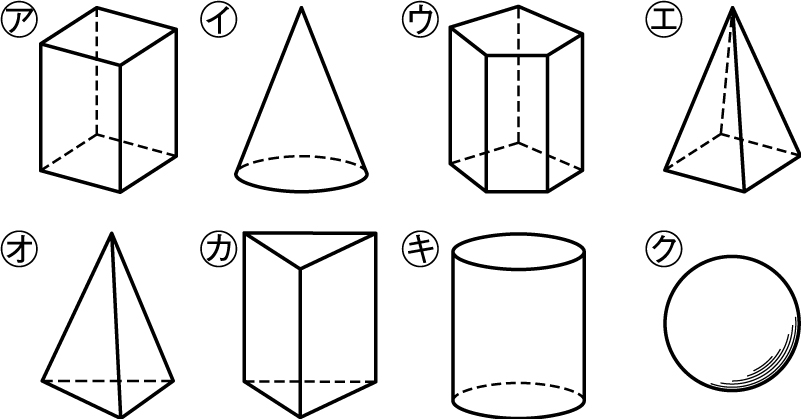
\includegraphics[height=40mm]{media/tu2.jpg}

\end{center}

(\text{\refstepcounter{skaunta}%
\arabic{skaunta}})\hspace{2.5pt}$\raise 0.2ex\hbox{\textcircled{\scriptsize{ア}}}, \, \raise 0.2ex\hbox{\textcircled{\scriptsize{ウ}}}, \, \raise 0.2ex\hbox{\textcircled{\scriptsize{エ}}}$の\ruby[g]{立体}{りったい}の\ruby[g]{名前}{なまえ}と、それが\ruby[g]{何面体}{なんめんたい}であるかを\ruby[g]{答}{こた}えなさい。

(\text{\refstepcounter{skaunta}%
\arabic{skaunta}})\hspace{2.5pt}$\raise 0.2ex\hbox{\textcircled{\scriptsize{オ}}}, \, \raise 0.2ex\hbox{\textcircled{\scriptsize{カ}}}$の\ruby[g]{立体}{りったい}の\ruby[g]{名前}{なまえ}と、\ruby[g]{側面}{そくめん}の\ruby[g]{形}{かたち}を\ruby[g]{答}{こた}えなさい。

(\text{\refstepcounter{skaunta}%
\arabic{skaunta}})\hspace{2.5pt}$\raise 0.2ex\hbox{\textcircled{\scriptsize{ク}}}$の\ruby[g]{立体}{りったい}の\ruby[g]{名前}{なまえ}を\ruby[g]{答}{こた}えなさい。

\setcounter{skaunta}{0}

\vfill

\noindent\fbox{\large\makebox[1em]{\text{\refstepcounter{kaunta}%
\arabic{kaunta}}}} \hspace{1pt}\ruby[g]{正四面体}{せいしめんたい}、\ruby[g]{正六面体}{せいろくめんたい}、\ruby[g]{正八面体}{せいはちめんたい}について、\ruby[g]{下}{した}の\ruby[g]{表}{ひょう}の\ruby[g]{空欄}{くうらん}をうめて、\ruby[g]{表}{ひょう}を\ruby[g]{完成}{かんせい}させなさい。

%
\begin{flushright}%
\footnotesize{<知・技$2 \times 4$点>}%
\end{flushright}%


\begin{center}
\def\@captype{figure}
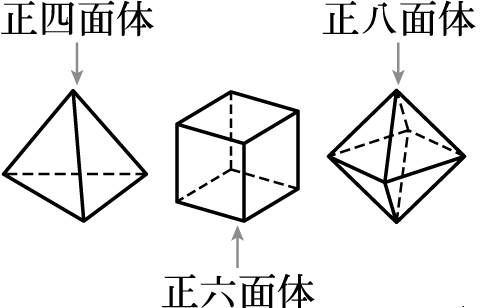
\includegraphics[height=40mm]{media/tu3.jpg}


\renewcommand{\arraystretch}{1.5}
\begin{tabular}{|c|c|c|c|}
\hline
 & \ruby[g]{面}{めん}の\ruby[g]{数}{かず} & \ruby[g]{辺}{へん}の数 &\ruby[g]{ 頂点}{ちょうてん}の\ruby[g]{数}{かず} \\
\hline
\ruby[g]{正四面体}{せいしめんたい} & (\text{\refstepcounter{skaunta}%
\arabic{skaunta}})\hspace{2.5pt}& 6 & 4\\
\hline
\ruby[g]{正六面体}{せいろくめんたい} & 6 & 12 & (\text{\refstepcounter{skaunta}%
\arabic{skaunta}})\hspace{2.5pt}\\
\hline
\ruby[g]{正八面体}{せいはちめんたい} & (\text{\refstepcounter{skaunta}%
\arabic{skaunta}})\hspace{2.5pt}& (\text{\refstepcounter{skaunta}%
\arabic{skaunta}})\hspace{2.5pt}& 6\\
\hline
\end{tabular}

\end{center}

\vfill

\newpage

\begin{multicols}{2}

\noindent\fbox{\large\makebox[1em]{\text{\refstepcounter{kaunta}%
\arabic{kaunta}}}} \hspace{1pt}\ruby[g]{右}{みぎ}の\ruby[g]{長方形}{ちょうほうけい}ABCDについて、\ruby[g]{線分}{せんぶん}ADと\ruby[g]{線分}{せんぶん}BCの\ruby[g]{関係}{かんけい}を、\ruby[g]{記号}{きごう}を\ruby[g]{使}{つか}って2\ruby[g]{通}{とお}りの\ruby[g]{方法}{ほうほう}で\ruby[g]{表}{あらわ}しなさい。

%
\begin{flushright}%
\footnotesize{<知・技$4$点>}%
\end{flushright}%


\columnbreak

\begin{center}
\def\@captype{figure}
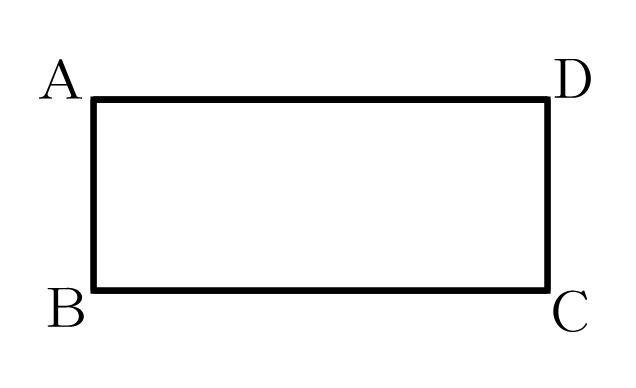
\includegraphics{media/image1.png}

\end{center}

\end{multicols}

\vspace*{\fill}

\begin{multicols}{2}

\noindent\fbox{\large\makebox[1em]{\text{\refstepcounter{kaunta}%
\arabic{kaunta}}}} \hspace{1pt}\ruby[g]{右}{みぎ}の\ruby[g]{図形}{ずけい}について、\ruby[g]{次}{つぎ}の\ruby[g]{問}{とい}に\ruby[g]{答}{こた}えなさい。

%
\begin{flushright}%
\footnotesize{<知・技$2 \times 2$点>}%
\end{flushright}%


\setcounter{skaunta}{0}

(\text{\refstepcounter{skaunta}%
\arabic{skaunta}})\hspace{2.5pt}\ruby[g]{三角形}{さんかくけい}を\ruby[g]{直線}{ちょくせん}$l$を\ruby[g]{対称}{たいしょう}の\ruby[g]{軸}{じく}として\ruby[g]{対称移動}{たいしょういどう}させた\ruby[g]{図形}{ずけい}をかきなさい。

\vspace*{\fill}

\columnbreak

\begin{center}
\def\@captype{figure}
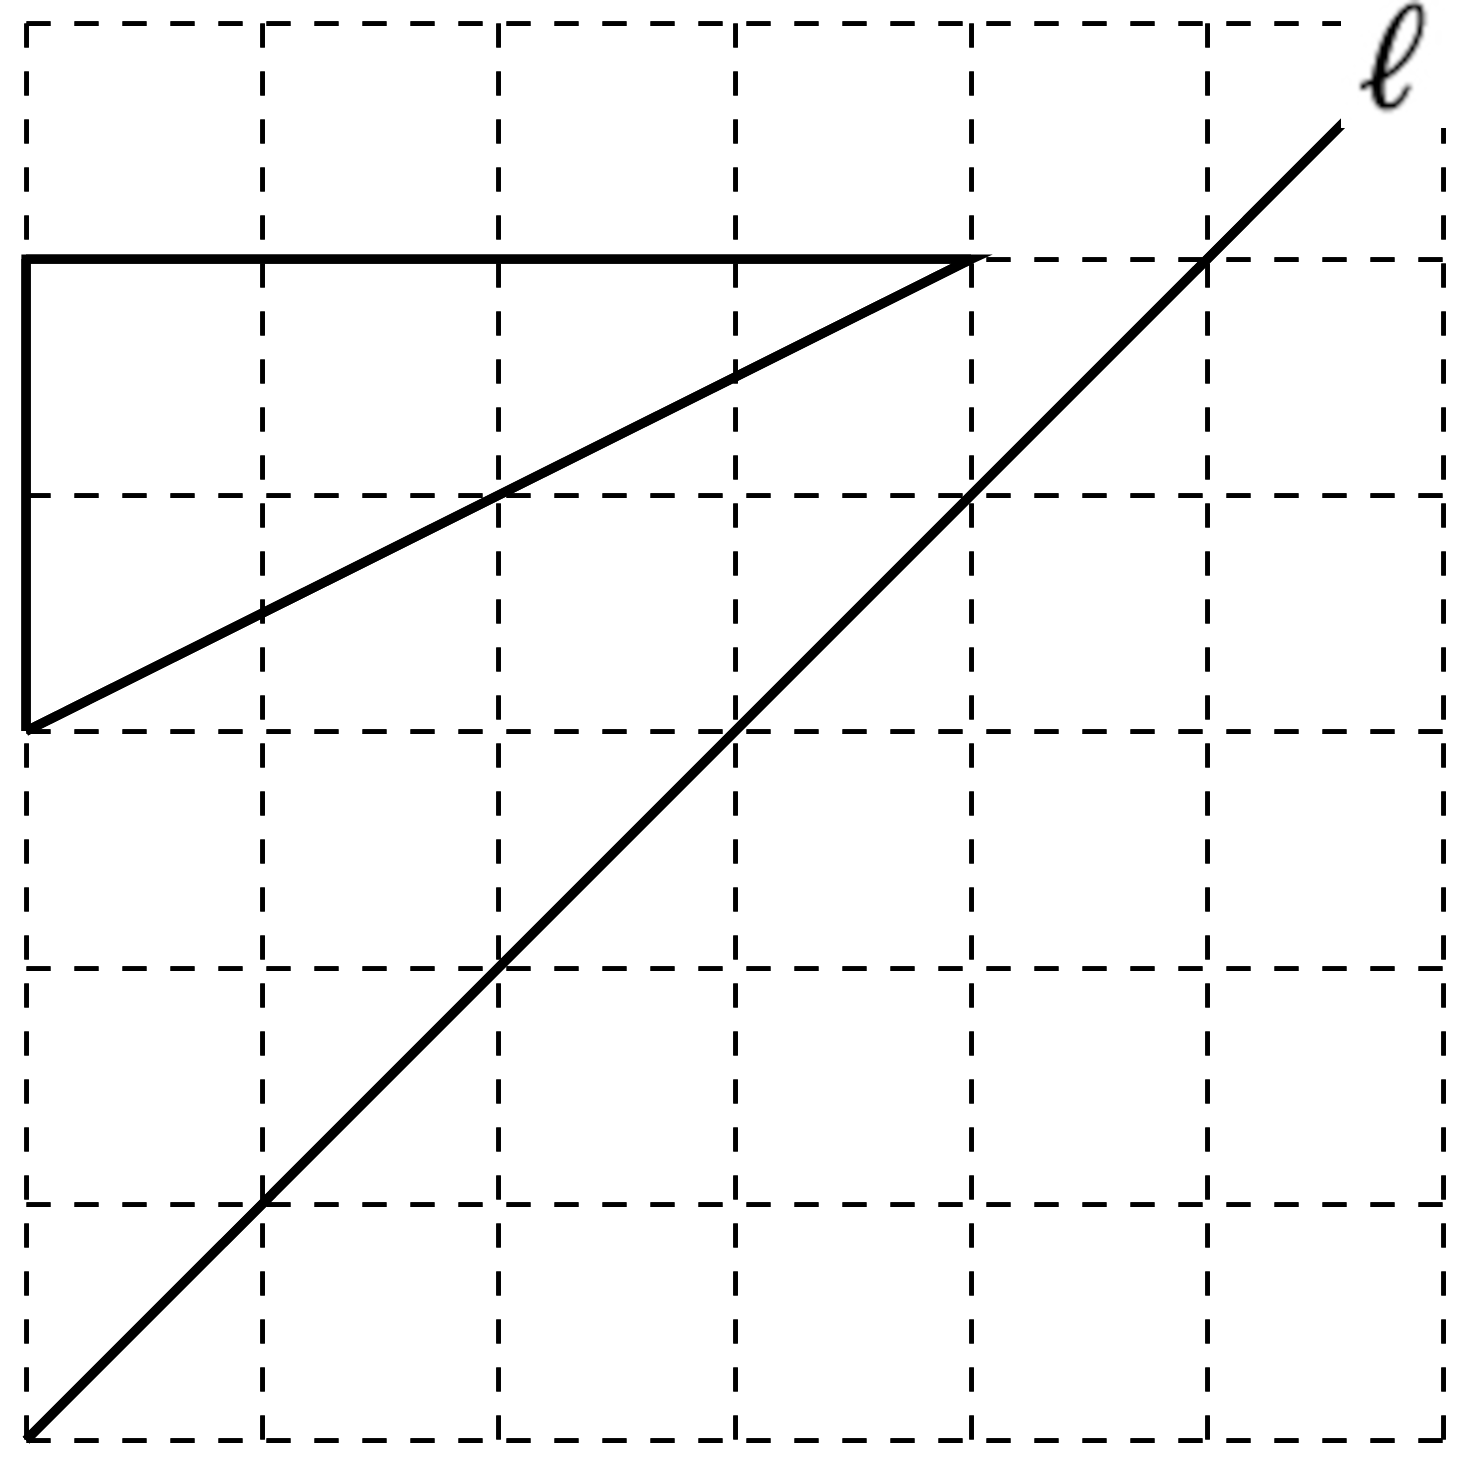
\includegraphics[width=30mm]{media/tu4.png}


\end{center}

\end{multicols}

\begin{multicols}{2}

(\text{\refstepcounter{skaunta}%
\arabic{skaunta}})\hspace{2.5pt}\ruby[g]{三角形}{さんかくけい}を\ruby[g]{点}{てん}Oを\ruby[g]{中心}{ちゅうしん}として$\ang{180}$\ruby[g]{回転移動}{かいてんいどう}させた\ruby[g]{図形}{ずけい}をかきなさい。

\vspace*{\fill}

\columnbreak

\begin{center}
\def\@captype{figure}
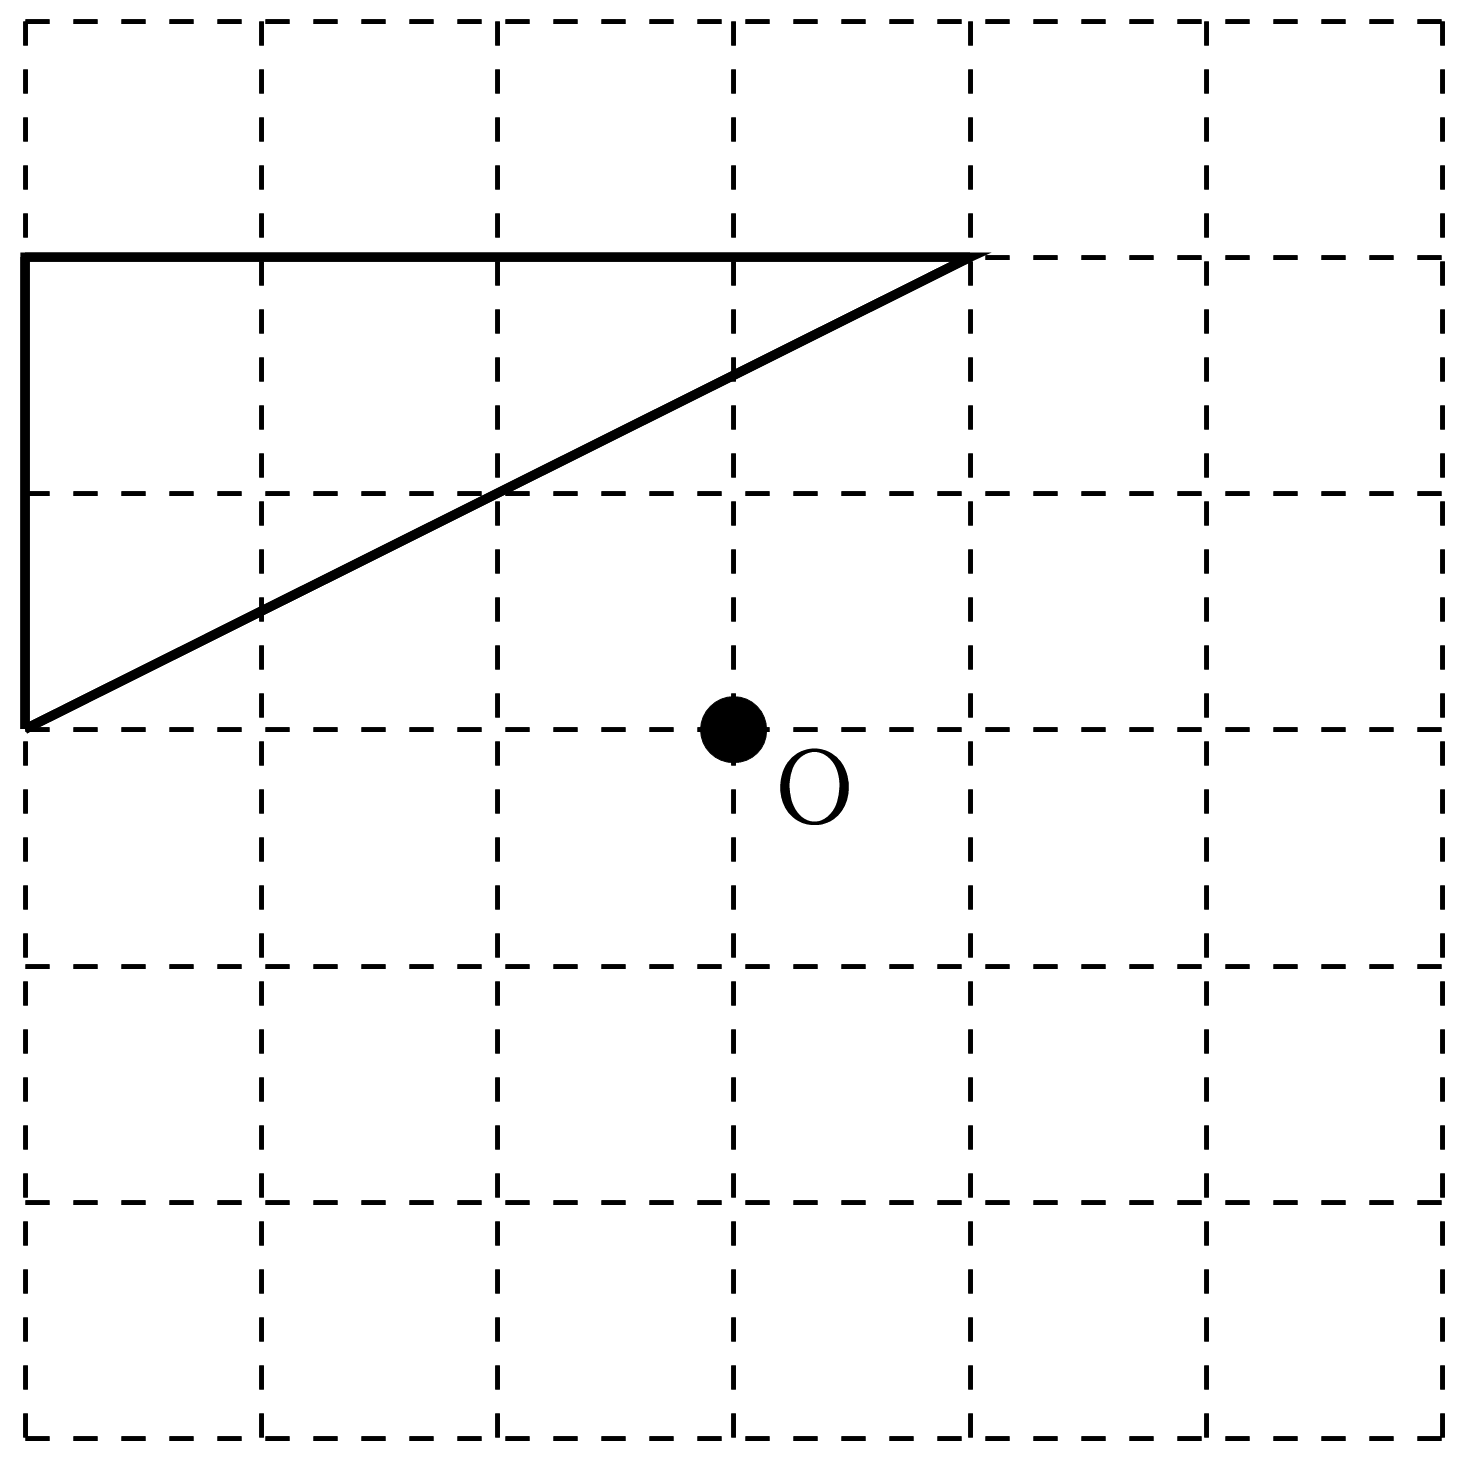
\includegraphics[width=30mm]{media/image3.png}

\end{center}

\end{multicols}

\begin{multicols}{2}

\vspace*{\fill}

\setcounter{skaunta}{0}
\noindent\fbox{\large\makebox[1em]{\text{\refstepcounter{kaunta}%
\arabic{kaunta}}}} \hspace{1pt}\ruby[g]{右}{みぎ}の\ruby[g]{図}{ず}の\ruby[g]{多角形}{たかくけい}ABCDEFは、1\ruby[g]{辺}{ぺん}が$2\si{cm}$の\ruby[g]{正六角形}{せいろっかくけい}で、\ruby[g]{点}{てん}Oは3つの\ruby[g]{対角線}{たいかくせん}の\ruby[g]{交点}{こうてん}です。

%
\begin{flushright}%
\footnotesize{<(1)(2)知・技$2 \times 2$点、(3)思・判・表2点>}%
\end{flushright}%


(\text{\refstepcounter{skaunta}%
\arabic{skaunta}})\hspace{2.5pt}$\triangle$EFOは$\triangle$BCOを、\ruby[g]{対角線}{たいかくせん}ADを\ruby[g]{対称}{たいしょう}の\ruby[g]{軸}{じく}として\ruby[g]{対称移動}{たいしょういどう}させた\ruby[g]{図形}{ずけい}とみることができます。このとき、ADとBFの\ruby[g]{関係}{かんけい}を\ruby[g]{式}{しき}で\ruby[g]{表}{あらわ}しなさい。

\columnbreak

\vspace*{\fill}

\begin{center}
\def\@captype{figure}
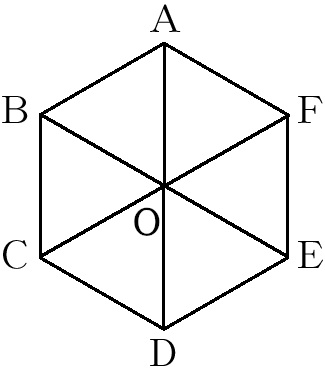
\includegraphics[width=30mm]{media/image5.png}

\end{center}

\vspace*{\fill}

\end{multicols}

\vspace*{\fill}

(\text{\refstepcounter{skaunta}%
\arabic{skaunta}})\hspace{2.5pt}$\triangle$BCOは、\ruby[g]{平行移動}{へいこういどう}だけで$\triangle$AOFに\ruby[g]{重}{かさ}ねることができます。このときの\ruby[g]{移動}{いどう}の\ruby[g]{距離}{きょり}は\ruby[g]{何}{なに}$\si{cm}$ですか。

\vspace*{\fill}

(\text{\refstepcounter{skaunta}%
\arabic{skaunta}})\hspace{2.5pt}$\triangle$BCOは、\ruby[g]{回転移動}{かいてんいどう}だけで$\triangle$AOFに\ruby[g]{重}{かさ}ねることができます。どのように\ruby[g]{移動}{いどう}したらよいか、その\ruby[g]{方法}{ほうほう}を\ruby[g]{説明}{せつめい}しなさい。

\vspace*{\fill}

\setcounter{skaunta}{0}

\newpage

\noindent\fbox{\large\makebox[1em]{\text{\refstepcounter{kaunta}%
\arabic{kaunta}}}} \hspace{1pt}\ruby[g]{次}{つぎ}の\ruby[g]{作図}{さくず}をしなさい。ただし、\ruby[g]{作図}{さくず}に\ruby[g]{用}{もち}いた\ruby[g]{線}{せん}は\ruby[g]{残}{のこ}しておくこと。

%
\begin{flushright}%
\footnotesize{<知・技$2 \times 5$点>}%
\end{flushright}%


(\text{\refstepcounter{skaunta}%
\arabic{skaunta}})\hspace{2.5pt}$\triangle$ABCで、\ruby[g]{辺}{へん}BCを\ruby[g]{底辺}{ていへん}としたときの\ruby[g]{高}{たか}さAP

\begin{center}
\def\@captype{figure}

\includegraphics[width=50mm]{media/image10.png}

\end{center}

(\text{\refstepcounter{skaunta}%
\arabic{skaunta}})\hspace{2.5pt}\ruby[g]{線分}{せんぶん}ABの\ruby[g]{中点}{ちゅうてん}M

\vspace{30mm}

\begin{center}
\def\@captype{figure}

\includegraphics[width=50mm]{media/image11.png}

\end{center}

(\text{\refstepcounter{skaunta}%
\arabic{skaunta}})\hspace{2.5pt}$\angle$AOBの\ruby[g]{二等分線}{にとうぶんせん}OC

\begin{center}
\def\@captype{figure}

\includegraphics[width=50mm]{media/image8.png}

\end{center}

(\text{\refstepcounter{skaunta}%
\arabic{skaunta}})\hspace{2.5pt}\ruby[g]{線分}{せんぶん}ABの\ruby[g]{垂直二等分線}{すいちょくにとうぶんせん}

\vspace{30mm}

\begin{center}
\def\@captype{figure}

\includegraphics[width=50mm]{media/image11.png}

\end{center}

(\text{\refstepcounter{skaunta}%
\arabic{skaunta}})\hspace{2.5pt}\ruby[g]{辺}{へん}AC, AB, BDに\ruby[g]{接}{せっ}する\ruby[g]{円}{えん}O

\vspace{15mm}

\begin{center}
\def\@captype{figure}
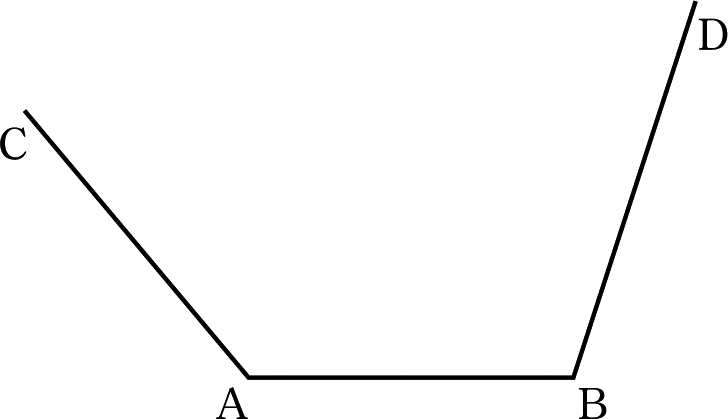
\includegraphics[width=50mm]{media/image191.png}

\end{center}

\newpage

\begin{multicols}{2}

\setcounter{skaunta}{0}
\noindent\fbox{\large\makebox[1em]{\text{\refstepcounter{kaunta}%
\arabic{kaunta}}}} \hspace{1pt}さやかさんは、\ruby[g]{右}{みぎ}の\ruby[g]{四角形}{しかくけい}\raise 0.2ex\hbox{\textcircled{\scriptsize{1}}}を、ある\ruby[g]{点}{てん}Oを\ruby[g]{回転}{かいてん}の\ruby[g]{中心}{ちゅうしん}として、\ruby[g]{回転移動}{かいてんいどう}させた\ruby[g]{図形}{ずけい}を\ruby[g]{並}{なら}べて、\ruby[g]{模様}{もよう}をつくることにしました。\ruby[g]{右}{みぎ}の\ruby[g]{四角形}{しかくけい}\raise 0.2ex\hbox{\textcircled{\scriptsize{2}}}は、\ruby[g]{四角形}{しかくけい}\raise 0.2ex\hbox{\textcircled{\scriptsize{1}}}を、\ruby[g]{点}{てん}Oを\ruby[g]{回転}{かいてん}の\ruby[g]{中心}{ちゅうしん}として\ruby[g]{時計回}{とけいまわ}りに$\ang{120}$\ruby[g]{移動}{いどう}させた\ruby[g]{図形}{ずけい}です。

%
\begin{flushright}%
\footnotesize{<(1)知・技2点、(2)思・判・表4点>}%
\end{flushright}%


\columnbreak

\begin{center}
\def\@captype{figure}
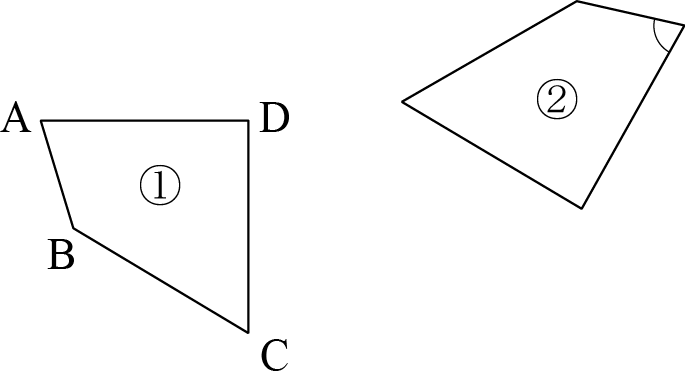
\includegraphics{media/image12.png}

\end{center}

\end{multicols}

(\text{\refstepcounter{skaunta}%
\arabic{skaunta}})\hspace{2.5pt}\ruby[g]{四角形}{しかくけい}\raise 0.2ex\hbox{\textcircled{\scriptsize{2}}}の\ruby[g]{印}{しるし}を\ruby[g]{付}{つ}けた\ruby[g]{角}{かく}(\def\@captype{figure}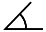
\includegraphics[scale=1.0]{media/image13.png})に\ruby[g]{対応}{たいおう}する\ruby[g]{角}{かく}を、\ruby[g]{次}{つぎ}のア$\sim$エの\ruby[g]{中}{なか}から\ruby[g]{選}{えら}び、\ruby[g]{記号}{きごう}で\ruby[g]{答}{こた}えなさい。

\begin{itemize}
\item[ア] $\angle$A
\item[イ] $\angle$B
\item[ウ] $\angle$C
\item[エ] $\angle$D
\end{itemize}



(\text{\refstepcounter{skaunta}%
\arabic{skaunta}})\hspace{2.5pt}さやかさんは、\ruby[g]{四角形}{しかくけい}\raise 0.2ex\hbox{\textcircled{\scriptsize{1}}}を\ruby[g]{四角形}{しかくけい}$\raise 0.2ex\hbox{\textcircled{\scriptsize{2}}}$に\ruby[g]{回転移動}{かいてんいどう}させた\ruby[g]{後}{あと}、\ruby[g]{回転}{かいてん}の\ruby[g]{中心}{ちゅうしん}Oの\ruby[g]{位置}{いち}が\ruby[g]{分}{わ}からなくなりました。\ruby[g]{回転}{かいてん}の\ruby[g]{中心}{ちゅうしん}Oの\ruby[g]{求}{もと}め\ruby[g]{方}{かた}を、「\ruby[g]{垂直二等分線}{すいちょくにとうぶんせん}」の\ruby[g]{言葉}{ことば}を\ruby[g]{使}{つか}って\ruby[g]{説明}{せつめい}しなさい。

\vspace{20mm}

\noindent\fbox{\large\makebox[1em]{\text{\refstepcounter{kaunta}%
\arabic{kaunta}}}} \hspace{1pt}$\ang{75}$を\ruby[g]{作図}{さくず}しなさい。

%
\begin{flushright}%
\footnotesize{<思・判・表5点>}%
\end{flushright}%


\newpage

\setcounter{skaunta}{0}
\noindent\fbox{\large\makebox[1em]{\text{\refstepcounter{kaunta}%
\arabic{kaunta}}}} \hspace{1pt}\ruby[g]{次}{つぎ}のおうぎ\ruby[g]{形}{がた}に\ruby[g]{関}{かん}する\ruby[g]{問}{とい}に\ruby[g]{答}{こた}えなさい。

%
\begin{flushright}%
\footnotesize{<知・技$2 \times 7$点>}%
\end{flushright}%


(\text{\refstepcounter{skaunta}%
\arabic{skaunta}})\hspace{2.5pt}\ruby[g]{半径}{はんけい}が$6\si{cm},$\ruby[g]{中心角}{ちゅうしんかく}が$\ang{30}$のおうぎ\ruby[g]{形}{がた}の\ruby[g]{面積}{めんせき}

\vspace{20mm}

(\text{\refstepcounter{skaunta}%
\arabic{skaunta}})\hspace{2.5pt}\ruby[g]{半径}{はんけい}が$10\si{cm},$\ruby[g]{中心角}{ちゅうしんかく}が$\ang{108}$のおうぎ\ruby[g]{形}{がた}の\ruby[g]{弧}{こ}の\ruby[g]{長}{なが}さ

\vspace{20mm}

(\text{\refstepcounter{skaunta}%
\arabic{skaunta}})\hspace{2.5pt}\ruby[g]{弧}{こ}の\ruby[g]{長}{なが}さが$10 \pi,$\ruby[g]{中心角}{ちゅうしんかく}が$\ang{120}$のおうぎ\ruby[g]{形}{がた}の\ruby[g]{面積}{めんせき}

\vspace{20mm}

(\text{\refstepcounter{skaunta}%
\arabic{skaunta}})\hspace{2.5pt}\ruby[g]{半径}{はんけい}が$12\si{cm},$\ruby[g]{面積}{めんせき}が$72 \pi \si{cm}^2$のおうぎ\ruby[g]{形}{がた}の\ruby[g]{中心角}{ちゅうしんかく}

\vspace{20mm}

(\text{\refstepcounter{skaunta}%
\arabic{skaunta}})\hspace{2.5pt}\ruby[g]{弧}{こ}の\ruby[g]{長}{なが}さが$6 \pi \si{cm}, $\ruby[g]{中心角}{ちゅうしんかく}が$\ang{120}$のおうぎ\ruby[g]{形}{がた}の\ruby[g]{半径}{はんけい}

\vspace{20mm}

(\text{\refstepcounter{skaunta}%
\arabic{skaunta}})\hspace{2.5pt}\ruby[g]{中心角}{ちゅうしんかく}が$\ang{90} \si{cm},$\ruby[g]{弧}{こ}の\ruby[g]{長}{なが}さが$9 \pi \si{cm}$のおうぎ\ruby[g]{形}{がた}の\ruby[g]{面積}{めんせき}

\vspace{20mm}

\begin{multicols}{2}

(\text{\refstepcounter{skaunta}%
\arabic{skaunta}})\hspace{2.5pt}\ruby[g]{右}{みぎ}の\ruby[g]{図}{ず}は、2つのおうぎ\ruby[g]{形}{がた}を\ruby[g]{組}{く}み\ruby[g]{合}{あ}わせたものである。\ruby[g]{色}{いろ}をつけた\ruby[g]{部分}{ぶぶん}について、\ruby[g]{次}{つぎ}のものを\ruby[g]{求}{もと}めなさい。

\columnbreak

\begin{center}
\def\@captype{figure}
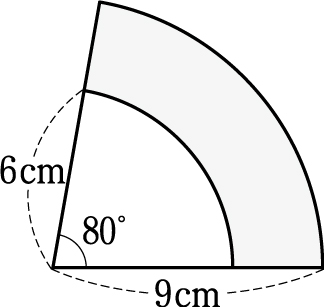
\includegraphics[height=30mm]{media/tu1.jpg}

\end{center}

\end{multicols}

\vfill

\newpage






















\end{flushleft}

\end{document}
